% !TEX program = xelatex
\documentclass[aspectratio=169]{beamer}
%%%%%%%%%%%%%%%%%%%%%%%%%%%%%%%%%%%%%%%%%%%%%%%%%%%%%%%%%%
% 文档类与全局设置
%%%%%%%%%%%%%%%%%%%%%%%%%%%%%%%%%%%%%%%%%%%%%%%%%%%%%%%%%%
% \documentclass[aspectratio=169]{beamer}
%tikz包
\usepackage{amsmath, amssymb, xcolor, tikz}
\usetikzlibrary{calc}  % 计算坐标
\usetikzlibrary{backgrounds}  % 背景支持（如果想使用 on background layer）
\usepackage[most]{tcolorbox}
\usepackage{xparse}

%字体设置
\usepackage{fontspec}
\usepackage{xeCJK}
\usepackage{unicode-math}
\usepackage{etoolbox} % 用于开关切换与核心排版补丁

% \newtoggle{fontBlackTheme}
% \togglefalse{fontBlackTheme}

\newcommand{\UseBlackFont}{\toggletrue{fontBlackTheme}}
\newcommand{\UseSongFont} { \togglefalse{fontBlackTheme}}

% ========================================================
% 【核心优化】字体全局控制解耦
% 拆分中英文字体设置，提供原子化命令，实现自由组合与扩展
% ========================================================
\newcommand{\SetENFont}[1]{%
  \setmainfont{#1}%
  \setsansfont{#1}%
  \setmonofont{#1}%
}
\newcommand{\SetCNFont}[1]{%
  \setCJKmainfont{#1}%
  \setCJKsansfont{#1}%
  \setCJKmonofont{#1}%
}
\newcommand{\SetMathFontConfig}[1]{%
  \setmathfont{#1}%
}

% 【新增】混合风格组合：中文黑体 + 英文新罗马
\newcommand{\UseHeiRomanFont}{%
  \SetENFont{Times New Roman}%
  \SetCNFont{Noto Sans CJK SC}%
  \SetMathFontConfig{TeX Gyre Termes Math}%
}

% 经典风格封装：全黑体
\newcommand{\ThemeBlackSans}{%
  \SetENFont{Liberation Sans}%
  \SetCNFont{Noto Sans CJK SC}%
  \SetMathFontConfig{TeX Gyre Termes Math}%
}

% 经典风格封装：全宋体/新罗马
\newcommand{\ThemeSongRoman}{%
  \SetENFont{Times New Roman}%
  \SetCNFont{Noto Serif CJK SC}%
  \SetMathFontConfig{TeX Gyre Termes Math}%
}

% \UseSongFont   % ← 这里启用“宋体+Times New Roman”主题
% \UseBlackFont  % ← 启用“黑体+Liberation Sans”主题

% %—— 根据开关选择字体（原逻辑保留，底层调用解耦命令更清爽） —— 
% \iftoggle{fontBlackTheme}{
%   \ThemeBlackSans
% }{
%   \ThemeSongRoman
% }
% 注意：若想完全摆脱开关直接使用组合，可以在这里直接调用 \UseHeiRomanFont 等命令覆盖上述设置

%------------------------------
% 伪代码环境
%------------------------------
% 引入算法宏包：ruled(顶部/底部画线), linesnumbered(显示行号), vlined(显示代码块垂线)
\usepackage[ruled,linesnumbered,vlined]{algorithm2e}

% 将 algorithm2e 默认的英文关键词替换为中文
% \SetKwInput{KwIn}{输入}
% \SetKwInput{KwOut}{输出}
% \SetAlgorithmName{算法}{算法}{算法列表}

%%%%%%%%%%%%%%%%%%%%%%%%%%%%%%%%%%%%%%%%%%%%%%%%%%%%%%%%%%
% 图形、色彩与数学设置
%%%%%%%%%%%%%%%%%%%%%%%%%%%%%%%%%%%%%%%%%%%%%%%%%%%%%%%%%%
\usepackage{tikz}
\usepackage[table]{xcolor}    % 表格色块
\usepackage{booktabs}         % 三线表格式
\usepackage{pgfplots}
\pgfplotsset{compat=1.18}

\usepackage{tcolorbox}
\usepackage{amsmath}
\usepackage{xcolor}

\usepackage{unicode-math}
\setmathfont{TeX Gyre Termes Math}
\setbeamercolor{block title}{fg=black,bg=gray!10}
\setbeamerfont{block title}{size=\normalsize,family=\rmfamily}


%%%%%%%%%%%%%%%%%%%%%%%%%%%%%%%%%%%%%%%%%%%%%%%%%%%%%%%%%%
% Beamer 主题与风格设置
%%%%%%%%%%%%%%%%%%%%%%%%%%%%%%%%%%%%%%%%%%%%%%%%%%%%%%%%%%
% 清除默认页眉与 frametitle 模板（后续自定义）
\setbeamertemplate{headline}{}
\setbeamertemplate{frametitle}{}
\setbeamertemplate{itemize item}[circle]

% 内外主题（可根据需求替换）
\useoutertheme[subsection=true]{miniframes} 
\useinnertheme{default}
\usecolortheme{default}

%%%%%%%%%%%%%%%%%%%%%%%%%%%%%%%%%%%%%%%%%%%%%%%%%%%%%%%%%%
% 颜色定义（可自定义调色板）
%%%%%%%%%%%%%%%%%%%%%%%%%%%%%%%%%%%%%%%%%%%%%%%%%%%%%%%%%%
\definecolor{lightpurple}{RGB}{134,0,106}
\definecolor{midpurple}{RGB}{112,0,95}
\definecolor{darkpurple}{RGB}{134,0,106}
\definecolor{myred}{RGB}{150,50,30}
\definecolor{mygreen}{RGB}{45,125,77}
\definecolor{mypurple}{RGB}{120,61,137}
\definecolor{myorange}{RGB}{190,88,32}
\definecolor{myitem}{RGB}{35,35,35}


%%%%%%%%%%%%%%%%%%%%%%%%%%%%%%%%%%%%%%%%%%%%%%%%%%%%%%%%%%
% 导航栏与页眉设置
%%%%%%%%%%%%%%%%%%%%%%%%%%%%%%%%%%%%%%%%%%%%%%%%%%%%%%%%%%
\makeatletter
% 设置顶部导航栏（用于章节、子章节导航）
\setbeamertemplate{headline}{%
  \begin{beamercolorbox}[wd=\paperwidth,ht=2ex,dp=1ex]{section in head/foot}
    \insertsectionnavigationhorizontal{\paperwidth}{}{}%
  \end{beamercolorbox}%
}
\setbeamercolor{section in head/foot}{bg=lightpurple, fg=white}
\setbeamercolor{subsection in head/foot}{bg=midpurple, fg=white}

% 自定义页眉
\setbeamertemplate{headline}{%
  \ifnum\value{framenumber}>1
    \ifx\insertframetitle\@empty
      % 【修复】即使没有标题，也撑开等量高度，防止正文排版上下跳动
      \rule{0pt}{0.9cm}
    \else
      % 视觉层：保持 overlay 不变
      \begin{tikzpicture}[remember picture,overlay]
        \node[anchor=west, font=\normalsize, text=black, xshift=0.2cm, yshift=-0.4cm]
              at (current page.north west){\insertframetitle};
        \draw[line width=1pt, color=midpurple]
              ([yshift=-0.7cm]current page.north west) -- ([yshift=-0.7cm]current page.north east);
      \end{tikzpicture}%
      % 【核心修复】物理占位层：告诉引擎顶部有 0.9cm 的安全距离（0.7cm线高 + 0.2cm呼吸空间）
      \rule{0pt}{0.2cm}%
    \fi
  \fi
}
\makeatother
%%%%%%%%%%%%%%%%%%%%%%%%%%%%%%%%%%%%%%%%%%%%%%%%%%%%%%%%%%
% 图注样式设置
%%%%%%%%%%%%%%%%%%%%%%%%%%%%%%%%%%%%%%%%%%%%%%%%%%%%%%%%%%
\usepackage{caption}
\setbeamerfont{caption}{size=\footnotesize}
\setbeamercolor{caption}{fg=black}
% 此处使用默认字体，确保中文统一为 Noto Sans CJK SC
\setbeamerfont{caption name}{size=\footnotesize}
\setbeamercolor{caption name}{fg=black}
\setbeamertemplate{caption}[numbered]
\renewcommand{\figurename}{图}

% 3. 调整浮动体（如 figure）与其上下正文之间的全局间距
\setlength{\intextsep}{6pt plus 2pt minus 2pt}

% \textfloatsep 适用于浮动到页面顶部 [t] 或底部 [b] 的图片与正文的间距
\setlength{\textfloatsep}{6pt plus 2pt minus 2pt}


%%%%%%%%%%%%%%%%%%%%%%%%%%%%%%%%%%%%%%%%%%%%%%%%%%%%%%%%%%
% 列表样式设置
%%%%%%%%%%%%%%%%%%%%%%%%%%%%%%%%%%%%%%%%%%%%%%%%%%%%%%%%%%
\makeatletter
% 一级列表 (大 item)
\def\@listi{\leftmargin\leftmargini
    \topsep 0.4em \@plus 0.1em \@minus 0.1em    % 缩小与上方正文间距
    \parsep 0pt                                 
    \itemsep 0.4em \@plus 0.2em \@minus 0.1ex}  % 【关键】从 1.0em 改为 0.4em
\let\@listI\@listi

% 二级列表 (小 item)
\def\@listii{\leftmargin\leftmarginii
    \topsep 0.2em \@plus 0.1em \@minus 0.1em 
    \parsep 0pt
    \itemsep 0.2em \@plus 0.1em \@minus 0.05ex} % 【关键】进一步压缩二级列表间距
\makeatother

% 三级列表 (更小的 item)
\def\@listiii{\leftmargin\leftmarginiii
    \topsep 0.1em
    \parsep 0pt
    \itemsep 0.2em}
\makeatother

% 自定义无序列表图标，采用 \raisebox 微调图标位置
\newcommand{\useBigCircleItem}{%
  \setbeamertemplate{itemize item}{\raisebox{0.3ex}{\tikz{\draw[myitem, fill=myitem] (0,0) circle (2pt);}}}%
  \setbeamertemplate{itemize subitem}{\raisebox{0.3ex}{\tikz{\draw[myitem, fill=myitem] (0,0) circle (2pt);}}}%
  \setbeamertemplate{itemize subsubitem}{\raisebox{0.3ex}{\tikz{\draw[myitem, fill=myitem] (0,0) circle (2pt);}}}%
}
\newcommand{\useSmallCircleItem}{%
  \setbeamertemplate{itemize item}{\raisebox{0.35ex}{\tikz{\draw[myitem, fill=myitem, opacity=0.8] (0,0) circle (1pt);}}}%
  \setbeamertemplate{itemize subitem}{\raisebox{0.35ex}{\tikz{\draw[myitem, fill=myitem, opacity=0.8] (0,0) circle (1pt);}}}%
  \setbeamertemplate{itemize subsubitem}{\raisebox{0.35ex}{\tikz{\draw[myitem, fill=myitem, opacity=0.8] (0,0) circle (1pt);}}}%
}
% 默认使用大圆圈
\useBigCircleItem

% 有序列表样式
\setbeamercolor{enumerate item}{fg=lightpurple}
\setbeamertemplate{enumerate item}{%
  \usebeamerfont*{enumerate item}%
  \color{enumerate item.fg}\insertenumlabel.%
}

%%%%%%%%%%%%%%%%%%%%%%%%%%%%%%%%%%%%%%%%%%%%%%%%%%%%%%%%%%
% 页脚设置
%%%%%%%%%%%%%%%%%%%%%%%%%%%%%%%%%%%%%%%%%%%%%%%%%%%%%%%%%%
\setbeamertemplate{footline}{%
  \ifnum\insertpagenumber>2
    \begin{tikzpicture}[remember picture,overlay]
      \node[fill=lightpurple, minimum width=0.3\paperwidth, minimum height={0.4cm+1pt}, anchor=south west]
           at ([xshift=-1pt,yshift=-1pt]current page.south west) (leftblock) {};
      \node[fill=midpurple, minimum width=0.6\paperwidth, minimum height={0.4cm+1pt}, anchor=south west]
           at ([xshift=0.3\paperwidth-1pt,yshift=-1pt]current page.south west) (midblock) {};
      \node[fill=lightpurple, minimum width={0.1\paperwidth+1pt}, minimum height={0.4cm+1pt}, anchor=south west]
           at ([xshift=0.9\paperwidth-1pt,yshift=-1pt]current page.south west) (rightblock) {};
      \node[anchor=center, yshift=0.5pt, font=\tiny, text=white] at (leftblock.center)
           {戴一冕 https://grokcv.site/};
      \node[anchor=center, yshift=0.5pt, font=\tiny, text=white] at (midblock.center)
           {大规模图像的多粒度目标检测};
      \node[anchor=center, yshift=0.5pt, font=\tiny, text=white] at (rightblock.center)
           {\insertframenumber};
    \end{tikzpicture}%
  \fi
}

%%%%%%%%%%%%%%%%%%%%%%%%%%%%%%%%%%%%%%%%%%%%%%%%%%%%%%%%%%
% 注释宏定义
%%%%%%%%%%%%%%%%%%%%%%%%%%%%%%%%%%%%%%%%%%%%%%%%%%%%%%%%%%
\newcounter{cornernotecounter}

% 修复跨页污染：每次进入新的 frame 时计数器清零
% (需要 \usepackage{etoolbox}，你前面的配置里已经加了)
\BeforeBeginEnvironment{frame}{\setcounter{cornernotecounter}{0}}

\newcommand{\cornernote}[1]{%
  \begin{tikzpicture}[remember picture, overlay]
    % 核心修复：根据当前计数器的值，动态计算 Y 轴高度。
    % 基础高度 0.45cm，每多一个注脚，整体向上偏移 0.35cm，防止文字重叠
    \node[anchor=south west, xshift=0.6cm, yshift={0.45cm + (\value{cornernotecounter}-1)*0.3cm}] 
      at (current page.south west) {%
      {\scriptsize\color{gray}\textsuperscript{\thecornernotecounter} #1}%
    };
  \end{tikzpicture}%
}

\newcommand{\cornerfootnote}[1]{%
  \stepcounter{cornernotecounter}% 删除了致命的空行
  \textsuperscript{\thecornernotecounter}%
  \cornernote{#1}%
}
%%%%%%%%%%%%%%%%%%%%%%%%%%%%%%%%%%%%%%%%%%%%%%%%%%%%%%%%%%
% 表格样式宏定义
%%%%%%%%%%%%%%%%%%%%%%%%%%%%%%%%%%%%%%%%%%%%%%%%%%%%%%%%%%
\newcommand{\PlainTable}[1]{%
  {\footnotesize
   \setlength{\tabcolsep}{6pt}%
   #1%
  }%
}
\newcommand{\ThreeLineTable}[1]{%
  {\footnotesize
   \setlength{\tabcolsep}{6pt}%
   #1%
  }%
}
\newcommand{\AltColorTable}[1]{%
  {\footnotesize
   \setlength{\tabcolsep}{6pt}%
   \rowcolors{2}{gray!20}{white}%
   #1%
   \rowcolors{2}{}{}%
  }%
}

%%%%%%%%%%%%%%%%%%%%%%%%%%%%%%%%%%%%%%%%%%%%%%%%%%%%%%%%%%
%强调块（适用于公式等）
%%%%%%%%%%%%%%%%%%%%%%%%%%%%%%%%%%%%%%%%%%%%%%%%%%%%%%%%%%
% 定义参数 key 和默认值
\pgfkeys{
  /BehindEqBox/.is family, /BehindEqBox,
  color/.initial = midpurple,
  border/.initial = 1pt,
  style/.initial = solid,
  padding/.initial = 2.8mm
}

% 定义命令：支持键值对参数 + 内容
\NewDocumentCommand{\BehindEqBox}{O{} m}{%
  % 加载参数
  \pgfkeys{/BehindEqBox, #1}

  \vspace{1em}
  \begin{center}
    \begin{tikzpicture}[remember picture, overlay]
      \node[inner sep=\pgfkeysvalueof{/BehindEqBox/padding}] (E) {#2};

      \coordinate (A) at ([xshift=-25pt]E.south west);
      \coordinate (B) at ([xshift=25pt]E.north east);

      \begin{pgfonlayer}{background}
        \filldraw[fill=\pgfkeysvalueof{/BehindEqBox/color}, opacity=0.1, rounded corners=0.35cm]
          (A) rectangle (B);

        \draw[
          line width=\pgfkeysvalueof{/BehindEqBox/border},
          draw=\pgfkeysvalueof{/BehindEqBox/color},
          opacity=0.2,
          rounded corners=0.35cm,
          \pgfkeysvalueof{/BehindEqBox/style}
        ] 
        (A) rectangle (B);
      \end{pgfonlayer}
    \end{tikzpicture}
  \end{center}
  \vspace{1em}
}


%%%%%%%%%%%%%%%%%%%%%%%%%%%%%%%%%%%%%%%%%%%%%%%%%%%%%%%%%%
%字体高亮块
%%%%%%%%%%%%%%%%%%%%%%%%%%%%%%%%%%%%%%%%%%%%%%%%%%%%%%%%%%
% 替换原 block 环境
\newtcolorbox{beamerblockbox}[3][]{%
  enhanced,
  breakable,
  colback=#2!10,             % 内容背景（透明度 80%）
  colframe=#2,               % 框颜色 = 标题栏颜色
  coltitle=white,            % 标题文字颜色
  fonttitle=\large,
  title=#3,
  boxed title style={
    colback=#2,
    top=2pt, bottom=2pt,
    left=2pt, right=2pt,
    sharp corners=northwest,
    sharp corners=northeast,
  },
  boxrule=0pt,
  arc=1.5mm,
  shadow={0pt}{-1pt}{1.5mm}{black!30},
  left=2pt, right=2pt,
  top=2pt, bottom=2pt,
  before skip=6pt,  % block与上文之间的空隙
  #1,
}

% 替换默认 beamer block 环境
\let\oldblock\block
\renewenvironment{block}[1]{\begin{beamerblockbox}{midpurple}{#1}}{\end{beamerblockbox}}

\let\oldalertblock\alertblock
\renewenvironment{alertblock}[1]{\begin{beamerblockbox}{myred}{#1}}{\end{beamerblockbox}}

\let\oldexampleblock\exampleblock
\renewenvironment{exampleblock}[1]{\begin{beamerblockbox}{myorange}{#1}}{\end{beamerblockbox}}


%%%%%%%%%%%%%%%%%%%%%%%%%%%%%%%%%%%%%%%%%%%%%%%%%%%%%%%%%%
% 封面页函数
%%%%%%%%%%%%%%%%%%%%%%%%%%%%%%%%%%%%%%%%%%%%%%%%%%%%%%%%%%
\usepackage{tikz}
\usetikzlibrary{calc, backgrounds}

\newcommand{\DrawCoverPage}{%
\begin{frame}
  \begin{tikzpicture}[remember picture, overlay]
    % 横幅中心位置
    \coordinate (bannercenter) at ([yshift=0.5cm]current page.center);

    % 横幅背景（高度 3.5cm）
    \node[fill=lightpurple, inner sep=0pt, outer sep=0pt, 
          minimum width=\paperwidth, 
          minimum height=3.5cm, 
          anchor=center] (banner) at (bannercenter) {};

    % 横幅上下两条线
    \path let \p1 = (banner.north), \p2 = (banner.south) in
      coordinate (topline) at (\x1, \y1+0.15cm)
      coordinate (bottomline) at (\x2, \y2-0.15cm);

    \draw[line width=0.4pt, draw=lightpurple] ([xshift=-0.5\paperwidth]topline) -- ([xshift=0.5\paperwidth]topline);
    \draw[line width=0.4pt, draw=lightpurple] ([xshift=-0.5\paperwidth]bottomline) -- ([xshift=0.5\paperwidth]bottomline);

    % 标题
    \node[text=white, 
          font=\fontsize{32}{36}\selectfont\bfseries, 
          text width=0.9\paperwidth, 
          align=center] at (bannercenter) {\mytitle};

    % 作者信息（胶囊形外框）
    \node[draw=lightpurple, fill=none, line width=0.5pt, 
          rounded corners=0.4cm, % 圆角固定
          minimum height=0.8cm,  % 高度写死
          inner xsep=20pt,       % 左右内边距
          text height=0.4cm,       % 保持中文英文一致高度
          text depth=0cm,      % 调整基线
          font=\Large] 
          at ([yshift=-2.7cm]current page.center) {\myauthor};

    % 图片部分
    \node[anchor=north, yshift=-0.35cm, xshift=-0.15cm] 
         at (current page.north) 
         {
\includegraphics[width=3.5cm]{image/Cover image/Logo.png}};

    \node[anchor=south west, xshift=-0.5cm, yshift=-0.5cm] 
         at (current page.south west) 
         {
\includegraphics[width=6cm]{image/Cover image/element_1.png}};

    \node[anchor=south east, xshift=0.5cm, yshift=-0.5cm] 
         at (current page.south east) 
         {
\includegraphics[width=5.5cm]{image/Cover image/element_2.png}};
  \end{tikzpicture}
\end{frame}
}

%使用大圆圈
\useSmallCircleItem

%%%%%%%%%%%%%%%%%%%%%%%%%%%%%%%%%%%%%%%%%%%%%%%%%%%%%%%%%%
% 动态自适应目录页宏定义
%%%%%%%%%%%%%%%%%%%%%%%%%%%%%%%%%%%%%%%%%%%%%%%%%%%%%%%%%%
\usepackage{pgffor} % 引入循环支持包 (通常tikz已包含，显式引入保平安)

% 定义计数器用于统计条目数量
\newcounter{toccount}

% =======================================================
% 命令: \DrawTOC[高亮项索引]{逗号分隔的标题列表}
% 示例: \DrawTOC[2]{背景介绍, 核心方法, 实验结果, 总结展望}
% 默认高亮第一项。如果不希望有高亮，可以传 [0]
% =======================================================
\newcommand{\DrawTOC}[2][1]{%
  \begin{frame}[plain]
    \begin{tikzpicture}[remember picture, overlay]
      
      % --- 左侧静态背景 (无需变动) ---
      \fill[lightpurple] (current page.south west) rectangle ([xshift=3.5cm]current page.north west);
      \fill[white, rounded corners=15pt]
        ([xshift=1.6cm, yshift=1.5cm]current page.south west) rectangle ([xshift=1cm, yshift=-1.5cm]current page.north east);

      % --- 左侧文字 ---
      \node[anchor=center, align=center, text=lightpurple] at ([xshift=3.3cm, yshift=0cm]current page.west) {
        {\fontsize{32}{40}\bfseries\selectfont 汇\hspace{0.1em}报} \\[0.2cm]
        {\fontsize{32}{40}\bfseries\selectfont 提\hspace{0.1em}纲} \\[0.2cm]
        \rule{0.8cm}{1.5pt} \\[0.2cm]
        {\fontsize{10}{12}\bfseries\selectfont CONTENTS}
      };

      % --- 右侧动态生成排版块 ---
      \begin{scope}[shift={([xshift=2cm, yshift=0cm]current page.center)}]
        
        \tikzstyle{block_base} = [minimum width=9.5cm, minimum height=1.2cm, font=\Large\bfseries\selectfont]
        \tikzstyle{block_active} = [block_base, fill=lightpurple, text=white]
        \tikzstyle{block_inactive} = [block_base, fill=gray!20, draw=gray!30, line width=0.5pt, text=black!60]

        % 1. 统计传入的标题总数
        \setcounter{toccount}{0}
        \foreach \x in {#2} { \stepcounter{toccount} }

        % 2. 核心数学计算：计算最顶部色块的 Y 坐标，确保整体在页面绝对居中
        % 色块高度1.2cm + 间距0.3cm = 跨度步长 1.5cm
        \pgfmathsetmacro{\starty}{(\thetoccount-1) * 1.6 / 2}

        % 3. 循环渲染每一个块
        \foreach \x [count=\xi] in {#2} {
          % 根据当前索引计算 Y 坐标: curr_y = start_y - (i-1)*1.5
          \pgfmathsetmacro{\curry}{\starty - (\xi-1)*1.6}
          
          % 判断是否为当前激活项
          \ifnum\xi=#1\relax
            \node[block_active]   at (0, \curry) {\x};
          \else
            \node[block_inactive] at (0, \curry) {\x};
          \fi
        }
        
      \end{scope}
    \end{tikzpicture}
  \end{frame}
}

%%%%%%%%%%%%%%%%%%%%%%%%%%%%%%%%%%%%%%%%%%%%%%%%%%%%%%%%%%
% 动态自适应目录页宏定义 - 极简列表版 (适应长标题与多条目)
%%%%%%%%%%%%%%%%%%%%%%%%%%%%%%%%%%%%%%%%%%%%%%%%%%%%%%%%%%
% =======================================================
% 命令: \DrawListTOC[高亮项索引]{逗号分隔的标题列表}
% 示例: \DrawListTOC[2]{第一项, 这是一个非常长的第二项标题会自动换行, 第三项}
% =======================================================
\newcommand{\DrawListTOC}[2][1]{%
  \begin{frame}[plain]
    \begin{tikzpicture}[remember picture, overlay]
      
      % --- 左侧静态背景与文本 (保持品牌视觉一致) ---
      \fill[lightpurple] (current page.south west) rectangle ([xshift=3.5cm]current page.north west);
      \fill[white, rounded corners=15pt]
        ([xshift=1.6cm, yshift=1.5cm]current page.south west) rectangle ([xshift=1cm, yshift=-1.5cm]current page.north east);

      \node[anchor=center, align=center, text=lightpurple] at ([xshift=3.3cm, yshift=0cm]current page.west) {
        {\fontsize{32}{40}\bfseries\selectfont 汇\hspace{0.1em}报} \\[0.2cm]
        {\fontsize{32}{40}\bfseries\selectfont 提\hspace{0.1em}纲} \\[0.2cm]
        \rule{0.8cm}{1.5pt} \\[0.2cm]
        {\fontsize{10}{12}\bfseries\selectfont CONTENTS}
      };

      % --- 右侧自适应列表排版 ---
      \begin{scope}[shift={([xshift=-1.5cm, yshift=0cm]current page.center)}]
        
        % 统计条目总数
        \setcounter{toccount}{0}
        \foreach \x in {#2} { \stepcounter{toccount} }

        % 计算起始 Y 坐标
        % 步长拉大到 1.8cm，为长标题自动换行预留充足的垂直呼吸空间
        \pgfmathsetmacro{\starty}{(\thetoccount-1) * 1.5 / 2}

        \foreach \x [count=\xi] in {#2} {
          \pgfmathsetmacro{\curry}{\starty - (\xi-1)*1.5}
          
          % 渲染逻辑：序号 + 竖线分隔符 + 文本
          \ifnum\xi=#1\relax
            % --- 当前高亮项 ---
            % 1. 序号 (不足10补0)
            \node[font=\Large\bfseries, text=lightpurple, anchor=east] at (-0.2, \curry) {\ifnum\xi<10 0\xi\else\xi\fi};
            % 2. 纵向引导线
            \draw[lightpurple, line width=1.5pt] (0.1, \curry+0.4) -- (0.1, \curry-0.4);
            % 3. 文本 (设定 text width=9.5cm，超过该宽度自动向下方折行，左对齐)
            \node[font=\Large\bfseries, text=black, align=left, text width=8cm, anchor=west] at (0.4, \curry) {\x};
          \else
            % --- 未激活项 ---
            % 1. 弱化序号
            \node[font=\Large\bfseries, text=gray!40, anchor=east] at (-0.2, \curry) {\ifnum\xi<10 0\xi\else\xi\fi};
            % 2. 弱化纵向线
            \draw[gray!30, line width=1pt] (0.1, \curry+0.4) -- (0.1, \curry-0.4);
            % 3. 弱化文本 (降低字重为常规，改变颜色)
            \node[font=\Large, text=gray!60, align=left, text width=9.5cm, anchor=west] at (0.4, \curry) {\x};
          \fi
        }
        
      \end{scope}
    \end{tikzpicture}
  \end{frame}
}



%%%%%%%%%%%%%%%%%%%%%%%%%%%%%%%%%%%%%%%%%%%%%%%%%%%%%%%%%%
% 参考文献样式
%%%%%%%%%%%%%%%%%%%%%%%%%%%%%%%%%%%%%%%%%%%%%%%%%%%%%%%%%%

% 设置参考文献条目的颜色
\setbeamercolor{bibliography item}{fg=lightpurple}
\setbeamercolor{bibliography entry author}{fg=black}
\setbeamercolor{bibliography entry title}{fg=black}
\setbeamercolor{bibliography entry location}{fg=gray}
\setbeamercolor{bibliography entry note}{fg=gray}

% 修改参考文献图标（默认是难看的小信封/小书本）
% 选项：text（显示数字）, item（显示小图标）, circle, square
\setbeamertemplate{bibliography item}[text]

% ============================================================
% 字体风格：适配 Windows 系统
% ============================================================
\SetENFont{Arial}
\SetCNFont{微软雅黑}
\SetMathFontConfig{TeX Gyre Termes Math}

% ============================================================
% 封面信息
% ============================================================
\newcommand{\mytitle}{面向单细胞数据的 ANN 检索系统}
\newcommand{\myauthor}{软件工程 第13组}

% ============================================================
% 修复页眉：[plain] 帧（目录页）不渲染页眉，防止上移
% ============================================================
\makeatletter
\setbeamertemplate{headline}{%
  \ifbeamer@plainframe
  \else
    \ifnum\value{framenumber}>1
      \ifx\insertframetitle\@empty
        \rule{0pt}{0.9cm}
      \else
        \begin{tikzpicture}[remember picture,overlay]
          \node[anchor=west, font=\normalsize, text=black, xshift=0.2cm, yshift=-0.4cm]
                at (current page.north west){\insertframetitle};
          \draw[line width=1pt, color=midpurple]
                ([yshift=-0.7cm]current page.north west) -- ([yshift=-0.7cm]current page.north east);
        \end{tikzpicture}%
        \rule{0pt}{0.2cm}%
      \fi
    \fi
  \fi
}
\makeatother

% ============================================================
% 页脚：项目信息
% ============================================================
\setbeamertemplate{footline}{%
  \ifnum\insertpagenumber>2
    \begin{tikzpicture}[remember picture,overlay]
      \node[fill=lightpurple, minimum width=0.25\paperwidth, minimum height={0.4cm+1pt}, anchor=south west]
           at ([xshift=-1pt,yshift=-1pt]current page.south west) (leftblock) {};
      \node[fill=midpurple, minimum width=0.55\paperwidth, minimum height={0.4cm+1pt}, anchor=south west]
           at ([xshift=0.25\paperwidth-1pt,yshift=-1pt]current page.south west) (midblock) {};
      \node[fill=lightpurple, minimum width={0.2\paperwidth+1pt}, minimum height={0.4cm+1pt}, anchor=south west]
           at ([xshift=0.8\paperwidth-1pt,yshift=-1pt]current page.south west) (rightblock) {};
      \node[anchor=center, yshift=0.5pt, font=\tiny, text=white] at (leftblock.center)
           {软件工程 第13组};
      \node[anchor=center, yshift=0.5pt, font=\tiny, text=white] at (midblock.center)
           {面向单细胞数据的 ANN 检索系统——中期汇报};
      \node[anchor=center, yshift=0.5pt, font=\tiny, text=white] at (rightblock.center)
           {\insertframenumber};
    \end{tikzpicture}%
  \fi
}

\begin{document}

\linespread{1.2}
\setlength{\parskip}{0.5em plus 0.2em minus 0.1em}

%%%%%%%%%%%%%%%%%%%%%%%%%%%%%%%%%%%%%%%%%%%%%%%%%%%%%%%%%%
% 封面页
%%%%%%%%%%%%%%%%%%%%%%%%%%%%%%%%%%%%%%%%%%%%%%%%%%%%%%%%%%
\DrawCoverPage

%%%%%%%%%%%%%%%%%%%%%%%%%%%%%%%%%%%%%%%%%%%%%%%%%%%%%%%%%%
% 目录页（4 大段）
%%%%%%%%%%%%%%%%%%%%%%%%%%%%%%%%%%%%%%%%%%%%%%%%%%%%%%%%%%
\DrawListTOC[1]{
  项目背景与系统架构,
  核心功能实现,
  RAG 检索与用户权限管理,
  总结与后续计划
}

%%%%%%%%%%%%%%%%%%%%%%%%%%%%%%%%%%%%%%%%%%%%%%%%%%%%%%%%%%
% 第1页：项目背景与目标
%%%%%%%%%%%%%%%%%%%%%%%%%%%%%%%%%%%%%%%%%%%%%%%%%%%%%%%%%%
\begin{frame}{项目背景与目标}

\begin{columns}[T]
  \begin{column}{0.50\textwidth}
    \fontsize{8}{10}\selectfont
    \textbf{项目背景}
    \begin{itemize}
      \item 单细胞测序产生\textbf{数十万个细胞}样本，每个细胞是一个\textbf{高维向量}
      \item 传统精确搜索在大规模高维数据上\textbf{效率极低}
      \item ANN（Approximate Nearest Neighbor）技术在\textbf{质量与速度之间取得平衡}
    \end{itemize}

    \vspace{0.5em}
    \textbf{系统目标}
    \begin{itemize}
      \item 全栈 Web 应用：数据上传 $\to$ 预处理 $\to$ 索引 $\to$ 检索 $\to$ 可视化
      \item 至少实现一种 ANN 算法，支持 Top-K 相似细胞搜索
      \item 返回完整细胞信息：名称、元数据、距离值、查询耗时
    \end{itemize}
  \end{column}

  \begin{column}{0.46\textwidth}
    \begin{figure}
      \centering
      % ================================================================
      % 【截图1】系统架构图
      % ================================================================
      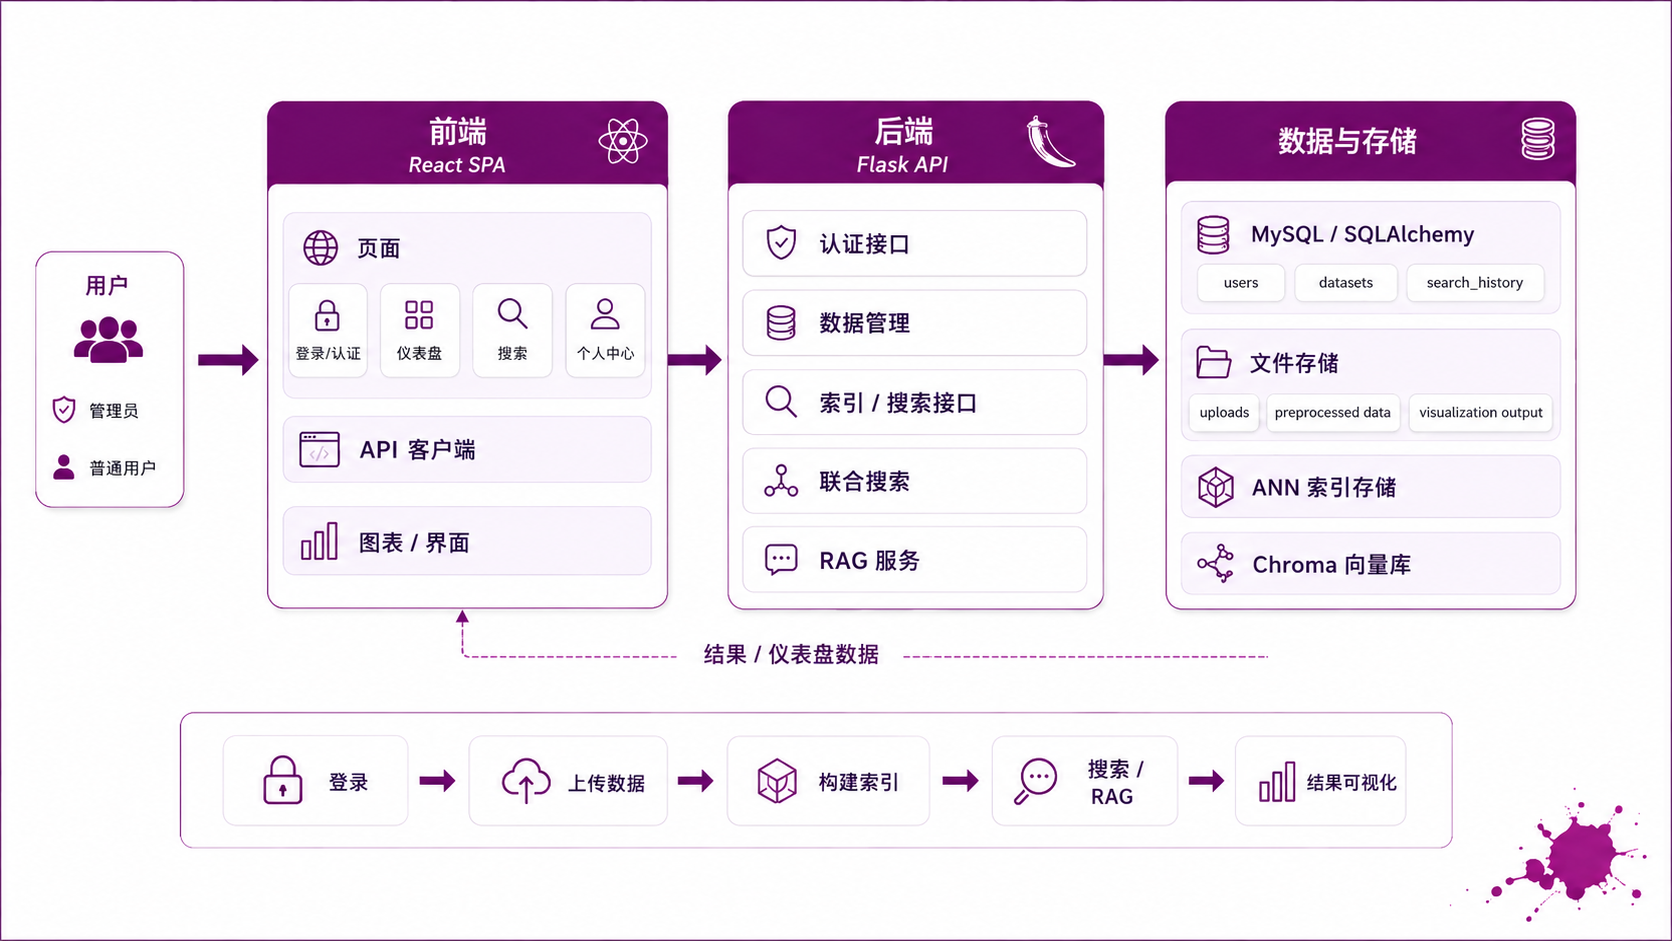
\includegraphics[width=\textwidth,keepaspectratio]{image/系统整体架构图.png}
      \caption{系统整体架构图}
    \end{figure}
  \end{column}
\end{columns}

\end{frame}

%%%%%%%%%%%%%%%%%%%%%%%%%%%%%%%%%%%%%%%%%%%%%%%%%%%%%%%%%%
% 第2页：系统架构与界面概览
%%%%%%%%%%%%%%%%%%%%%%%%%%%%%%%%%%%%%%%%%%%%%%%%%%%%%%%%%%
\begin{frame}{系统架构与界面概览}

\begin{columns}[T]
  \begin{column}{0.46\textwidth}
    \fontsize{8}{10}\selectfont
    \centering
    \textbf{技术栈}
    \vspace{0.3em}
    \ThreeLineTable{%
      \begin{tabular}{ll}
        \toprule
        \textbf{层级} & \textbf{技术} \\
        \midrule
        前端 & React 18 + MUI 5 + Recharts \\
        后端 & Flask 2.3 + JWT \\
        ANN & FAISS / Annoy / ChromaDB \\
        存储 & MySQL + 本地文件系统 \\
        \bottomrule
      \end{tabular}
    }

    \vspace{0.5em}
    \textbf{Dashboard 仪表盘说明}
    \begin{itemize}
      \item 右侧为系统主界面，提供\textbf{数据管理}与\textbf{索引管理}两个核心入口
      \item 概览卡片实时显示数据集数量、索引数量及最近搜索活动
      \item 导航栏支持中英文切换、深色/浅色主题切换
    \end{itemize}
  \end{column}

  \begin{column}{0.50\textwidth}
    \begin{figure}
      \centering
      % ================================================================
      % 【截图2】Dashboard 主界面
      % ================================================================
      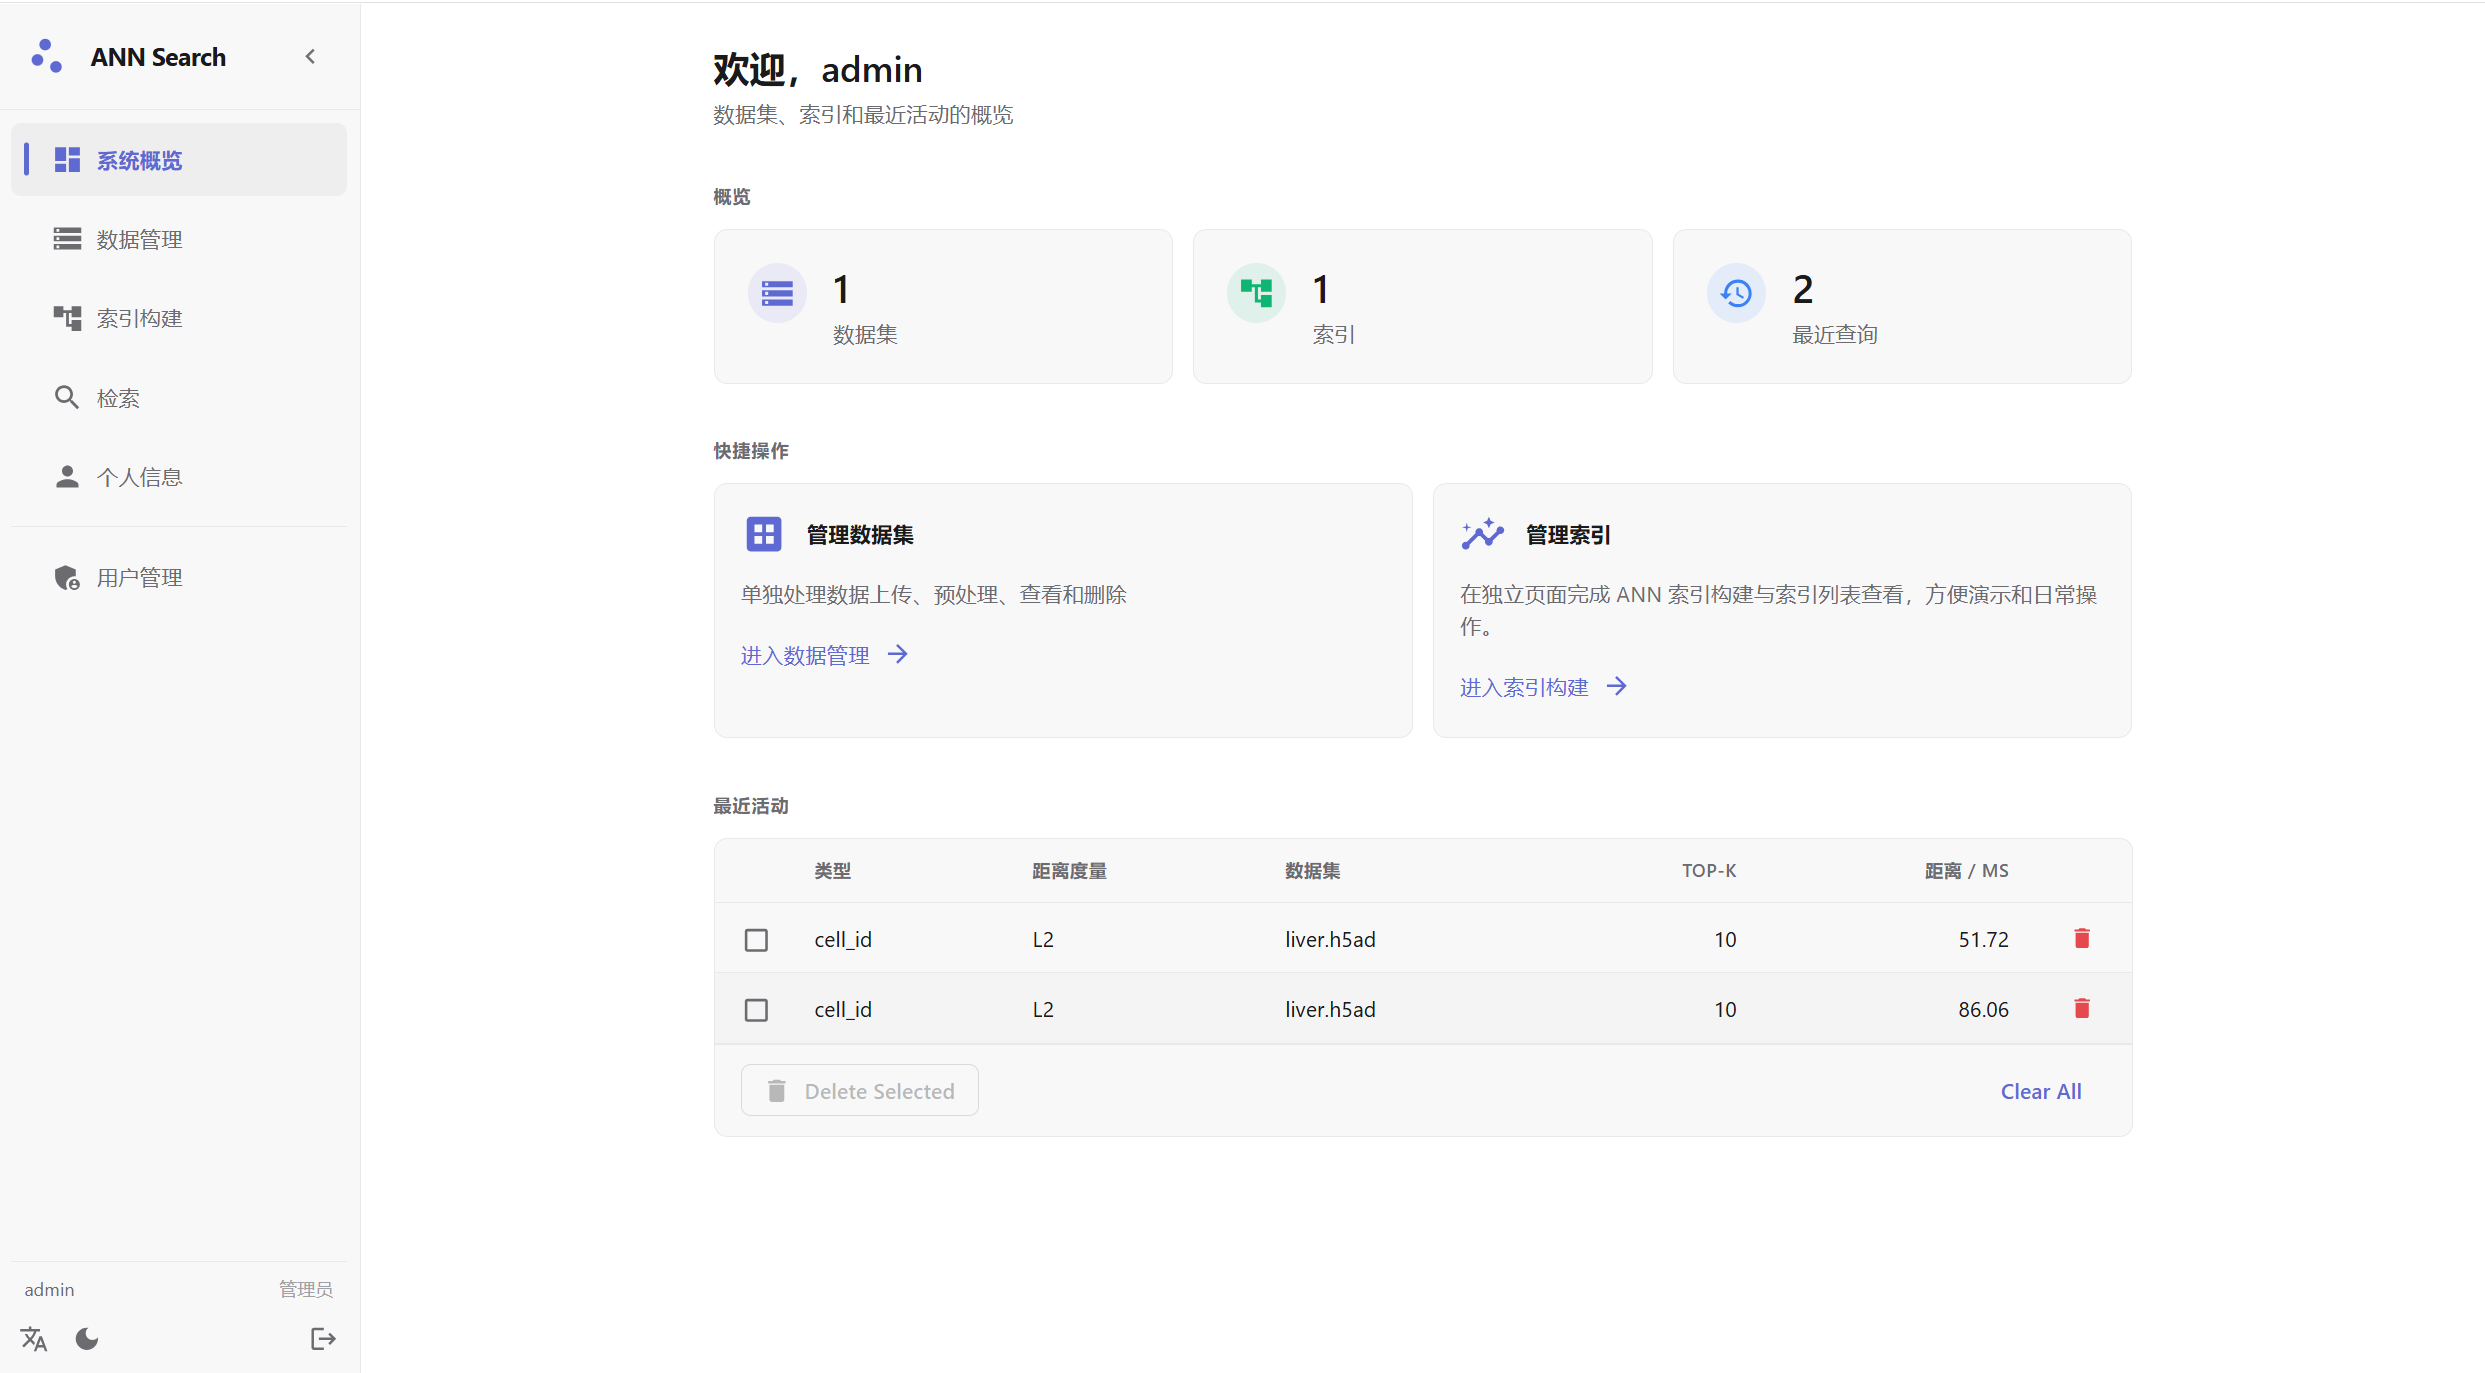
\includegraphics[width=\textwidth,keepaspectratio]{image/Dashboard 主界面.png}
      \caption{Dashboard 主页}
    \end{figure}
  \end{column}
\end{columns}

\end{frame}

%%%%%%%%%%%%%%%%%%%%%%%%%%%%%%%%%%%%%%%%%%%%%%%%%%%%%%%%%%
% 过渡页：核心功能实现
%%%%%%%%%%%%%%%%%%%%%%%%%%%%%%%%%%%%%%%%%%%%%%%%%%%%%%%%%%
\DrawTOC[2]{
  项目背景与系统架构,
  核心功能实现,
  RAG 检索与用户权限管理,
  总结与后续计划
}

% ================================================================
% 课程要求 1/6：单细胞数据读取
% ================================================================
\begin{frame}{单细胞数据读取}

\begin{columns}[T]
  \begin{column}{0.45\textwidth}
    \fontsize{8}{10}\selectfont
    \textbf{支持的数据格式}
    \begin{itemize}
      \item \textbf{CSV / TSV}：通用表格格式
      \item \textbf{HDF5 (.h5)}：通用层级数据格式
      \item \textbf{H5AD (.h5ad)}：AnnData 格式，单细胞数据标准
    \end{itemize}

    \vspace{0.5em}
    \textbf{课程数据适配}
    \begin{itemize}
      \item 优先读取 \texttt{obsm["X\_pca"]} 作为检索向量
      \item \texttt{obs} 元数据作为细胞标签（cell\_type、disease 等）
      \item 支持 UMAP / t-SNE 坐标用于可视化
    \end{itemize}

    \begin{alertblock}{$\checkmark$ 课程要求 1/6}
      单细胞数据读取
    \end{alertblock}
  \end{column}

  \begin{column}{0.52\textwidth}
    \begin{figure}
      \centering
      % ================================================================
      % 【截图3】数据管理界面全貌
      % ================================================================
      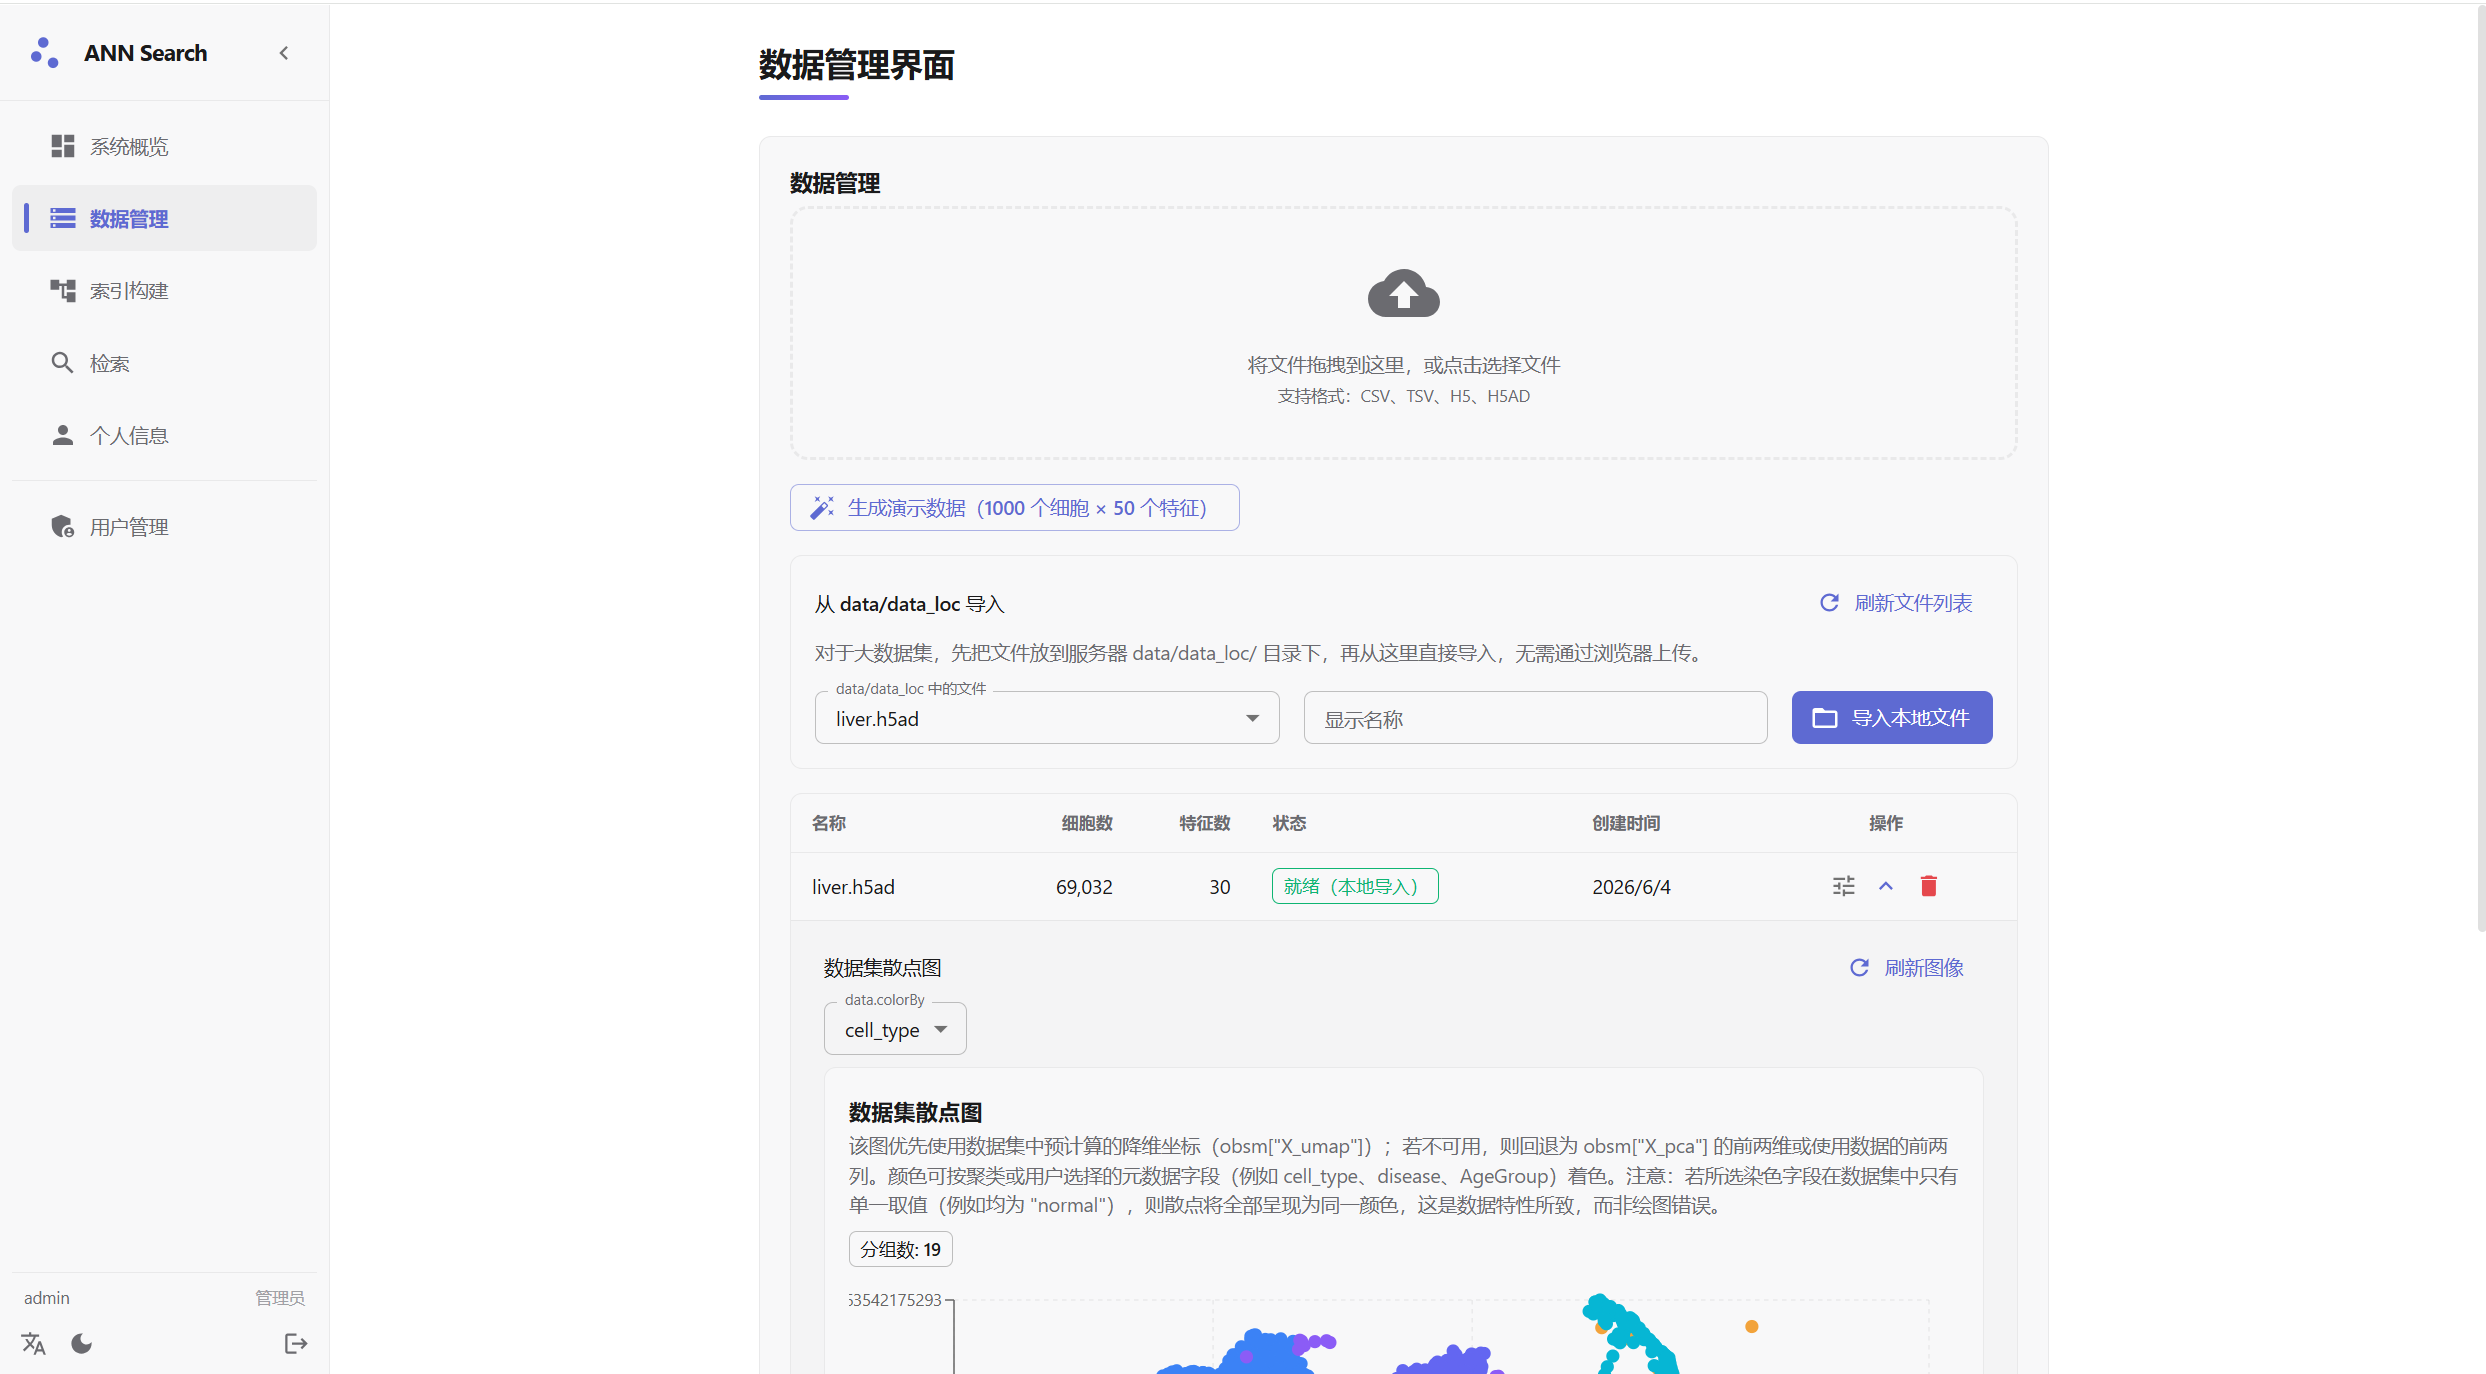
\includegraphics[width=\textwidth,keepaspectratio]{image/数据管理界面全貌.png}
      \caption{数据管理界面全貌}
    \end{figure}
  \end{column}
\end{columns}

\end{frame}

% ================================================================
% 课程要求 2/6：数据向量化表示
% ================================================================
\begin{frame}{数据向量化表示}

\begin{columns}[T]
  \begin{column}{0.45\textwidth}
    \fontsize{8}{10}\selectfont
    \vspace{1em}

    \textbf{向量化流程}
    \begin{itemize}
      \item 每个细胞 $\to$ 一个高维向量（PCA 降维后 50--100 维）
      \item 课程数据：直接使用 \texttt{obsm["X\_pca"]} 预计算 PCA 嵌入
      \item Demo 数据：随机生成可调维度的高斯分布向量
      \item 数据上传后自动解析，提取细胞名、特征名、元数据
    \end{itemize}

    \begin{alertblock}{$\checkmark$ 课程要求 2/6}
      数据向量化表示
    \end{alertblock}
  \end{column}

  \begin{column}{0.52\textwidth}
    \begin{figure}
      \centering
      % ================================================================
      % 【截图4】数据上传结果
      % ================================================================
      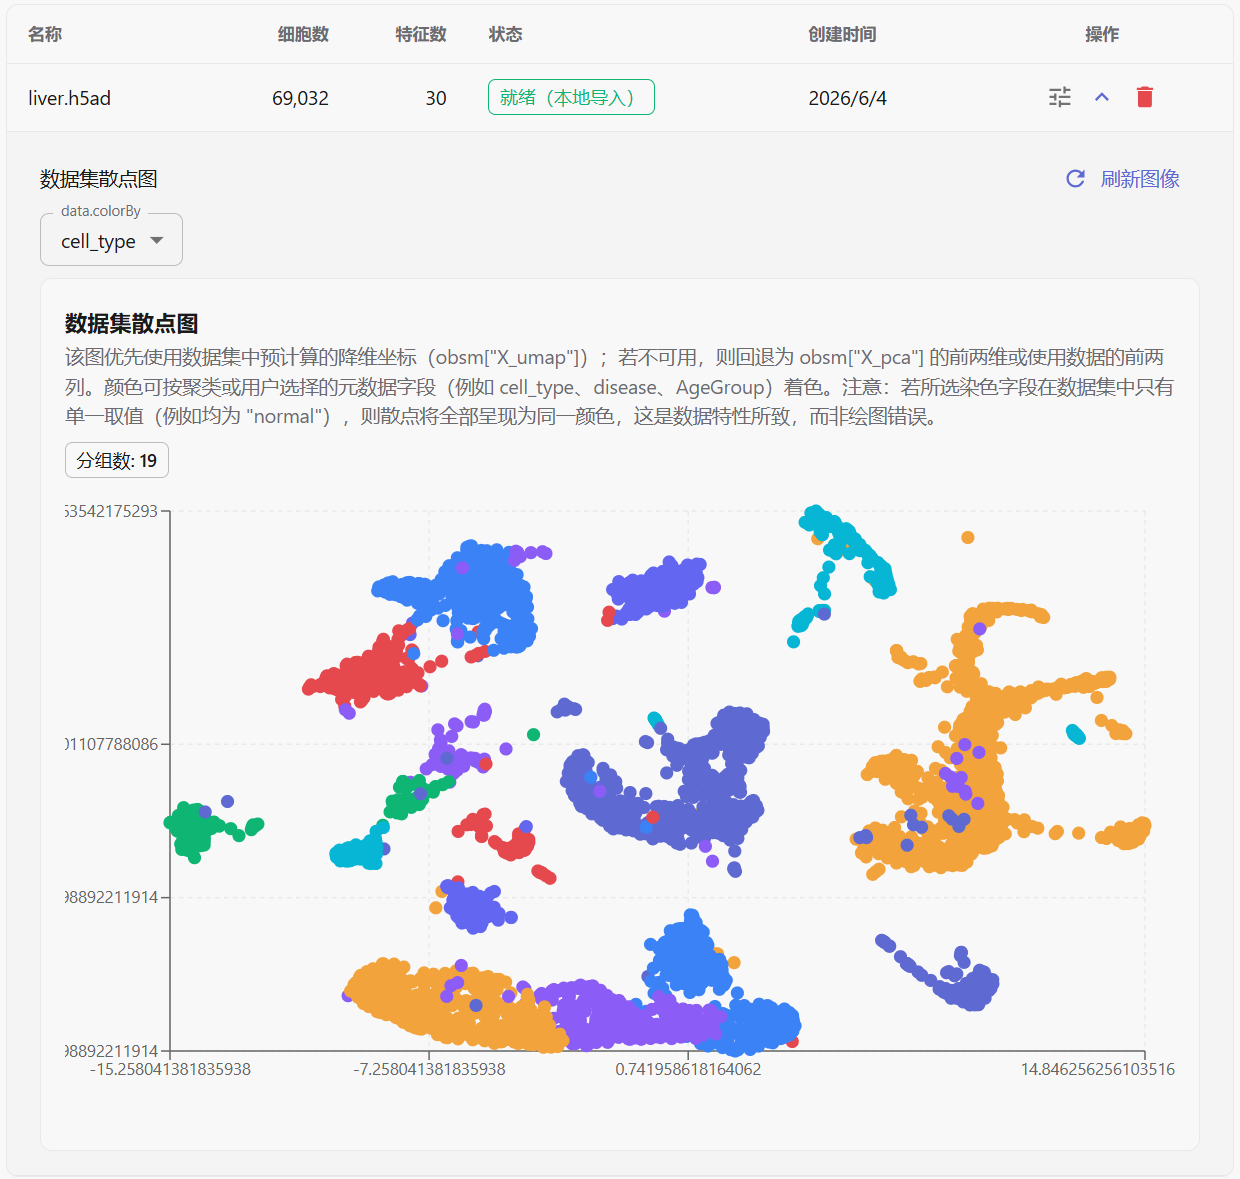
\includegraphics[width=\textwidth,keepaspectratio]{image/数据向量化结果.png}
      \caption{数据向量化结果}
    \end{figure}
  \end{column}
\end{columns}

\end{frame}

% ================================================================
% 数据预处理
% ================================================================
\begin{frame}{数据预处理}

\begin{columns}[T]
  \begin{column}{0.45\textwidth}
    \fontsize{8}{10}\selectfont
    \textbf{两种预处理方式}
    \begin{itemize}
      \item \textbf{L2 归一化}（按细胞）：每行缩放至单位范数
      \item \textbf{标准化}（按特征）：每列 z-score 标准化
    \end{itemize}

    \vspace{0.5em}
    \textbf{预处理特性}
    \begin{itemize}
      \item 原始数据保留在 \texttt{data\_web}，预处理副本写入 \texttt{data\_pre}
      \item 预处理后自动切换存储位置，检索与索引构建使用处理后的数据
      \item 数据集状态标签实时更新（如 ``preprocessed (L2 normalized)''）
    \end{itemize}
  \end{column}

  \begin{column}{0.52\textwidth}
    \begin{figure}
      \centering
      % ================================================================
      % 【截图5】预处理操作界面
      % ================================================================
      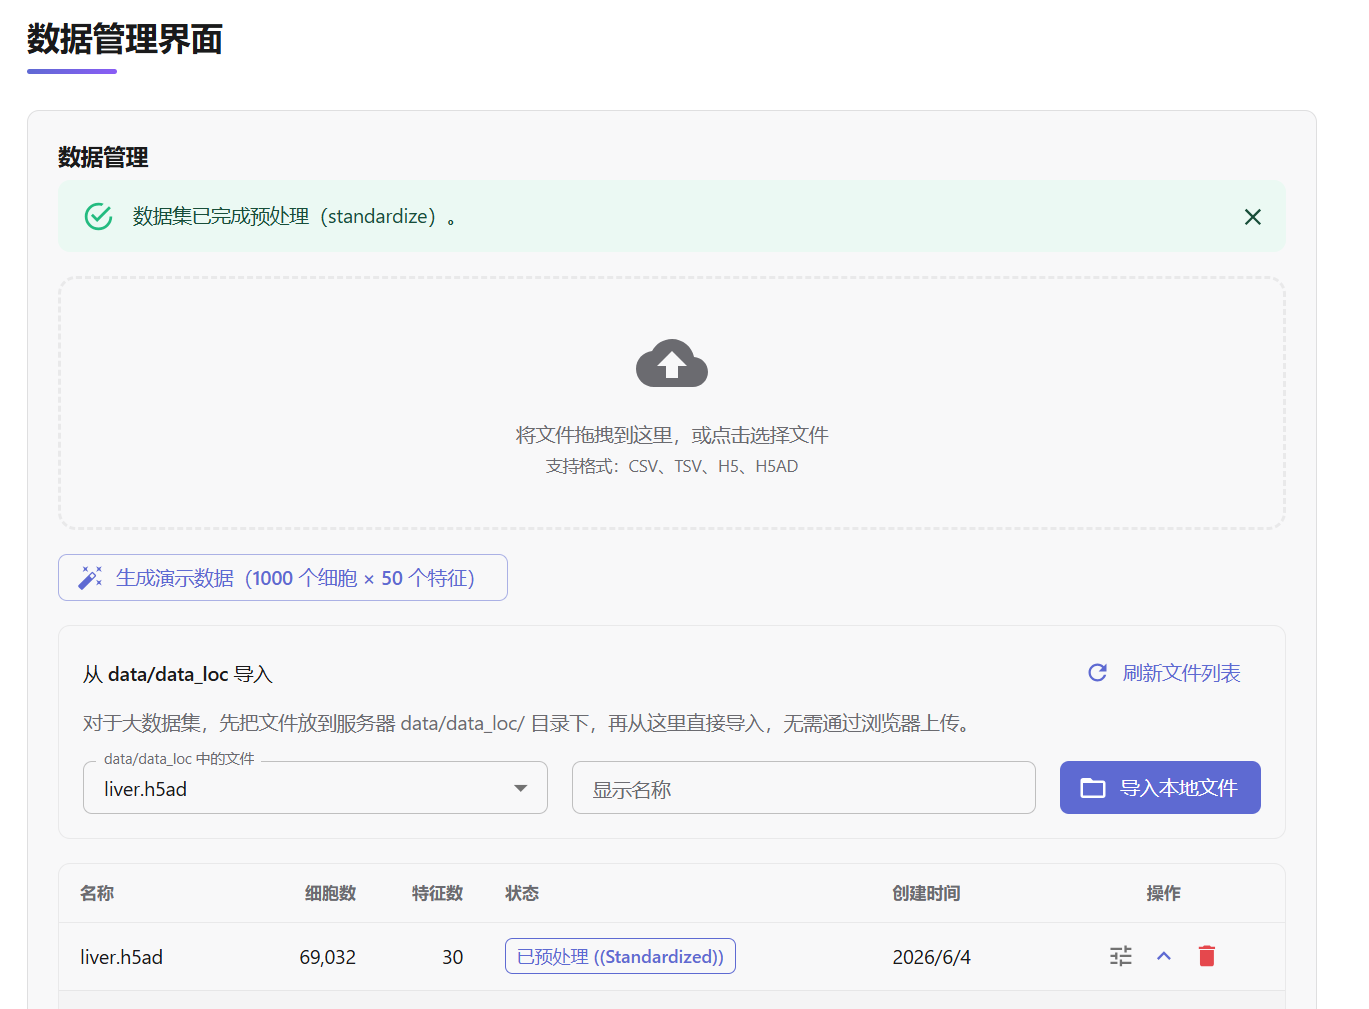
\includegraphics[width=\textwidth,keepaspectratio]{image/数据预处理.png}
      \caption{数据预处理}
    \end{figure}
  \end{column}
\end{columns}

\end{frame}

% ================================================================
% 课程要求 3/6：ANN 索引构建
% ================================================================
\begin{frame}{ANN 索引构建}

\begin{columns}[T]
  \begin{column}{0.42\textwidth}
    \fontsize{8}{10}\selectfont
    \vspace{1.2em}

    \textbf{构建流程}
    \begin{itemize}
      \item 选择已上传的数据集
      \item 选择索引类型：FAISS Flat、FAISS IVF、Annoy
      \item 选择距离度量：L2 / Cosine / Inner Product
      \item 一键构建，自动保存到磁盘
    \end{itemize}

    \vspace{0.5em}
    \textbf{索引管理}
    \begin{itemize}
      \item 索引列表展示：类型、度量、细胞数、特征数、构建耗时
      \item 支持查看详情、删除索引
      \item 索引文件保存在 \texttt{backend/storage/indices/}
    \end{itemize}

    \begin{alertblock}{$\checkmark$ 课程要求 3/6}
      ANN 索引构建
    \end{alertblock}
  \end{column}

  \begin{column}{0.55\textwidth}
    \begin{figure}
      \centering
      % ================================================================
      % 【截图6】索引构建表单
      % ================================================================
      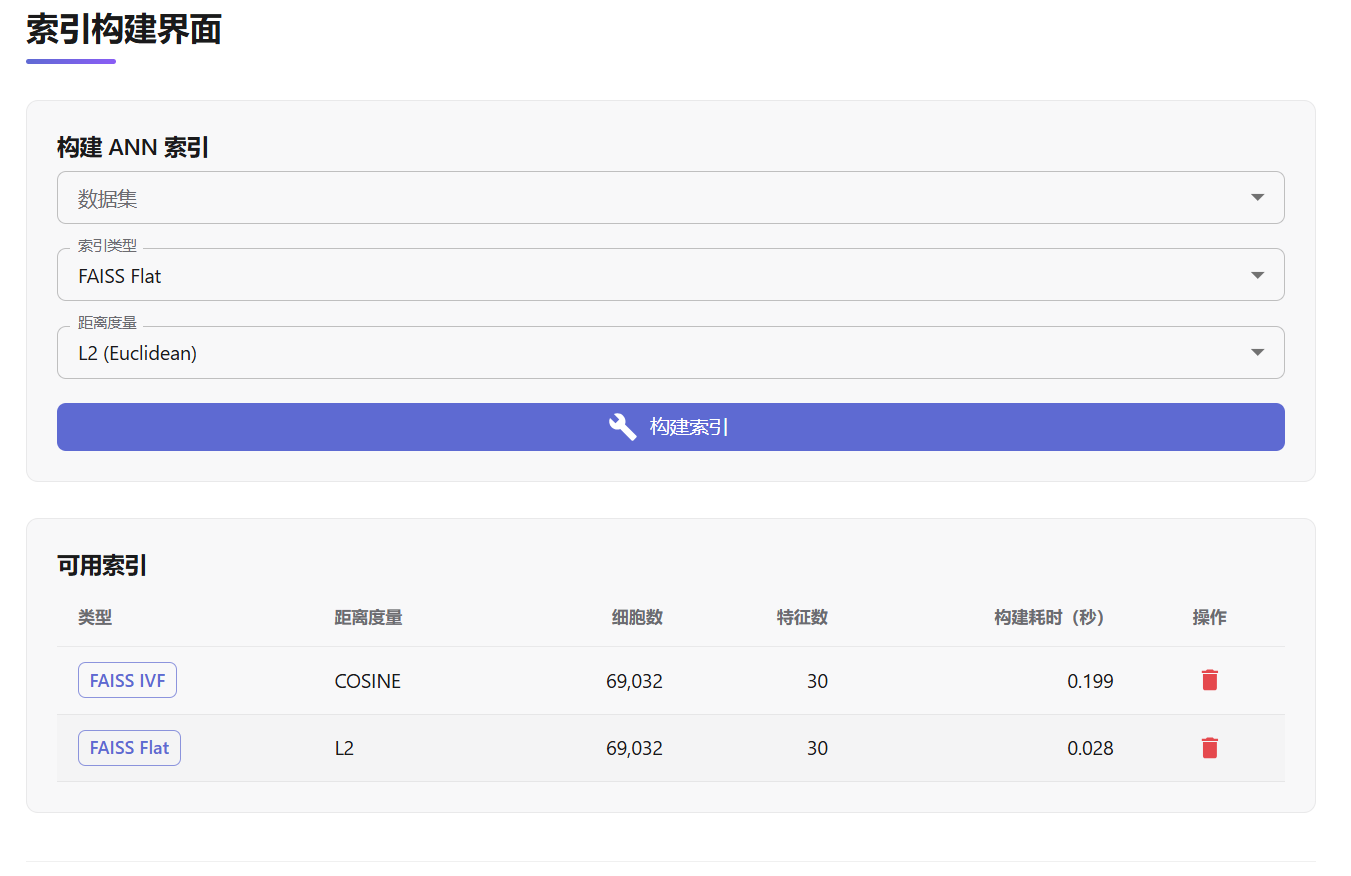
\includegraphics[width=\textwidth,keepaspectratio]{image/索引构件界面.png}
      \caption{索引构建界面}
    \end{figure}
  \end{column}
\end{columns}

\end{frame}

% ================================================================
% 联合索引管理
% ================================================================
\begin{frame}{联合索引管理}

\begin{columns}[T]
  \begin{column}{0.42\textwidth}
    \fontsize{8}{10}\selectfont
    \vspace{1.5em}

    \textbf{联合索引（Joint Index）}
    \begin{itemize}
      \item 基于 \textbf{ChromaDB HNSW}，支持多数据集合并为单一索引
      \item 跨数据集检索：一次查询，覆盖多个数据集
      \item 构建时自动将各数据集向量写入 ChromaDB Collection
    \end{itemize}

    \vspace{0.5em}
    \textbf{功能}
    \begin{itemize}
      \item 独立管理界面：构建表单、索引列表、删除
      \item 支持自然语言查询（配合 RAG 模块）
      \item 查询返回跨数据集 Top-K 结果
    \end{itemize}
  \end{column}

  \begin{column}{0.55\textwidth}
    \begin{figure}
      \centering
      % ================================================================
      % 【截图7】联合索引管理
      % ================================================================
      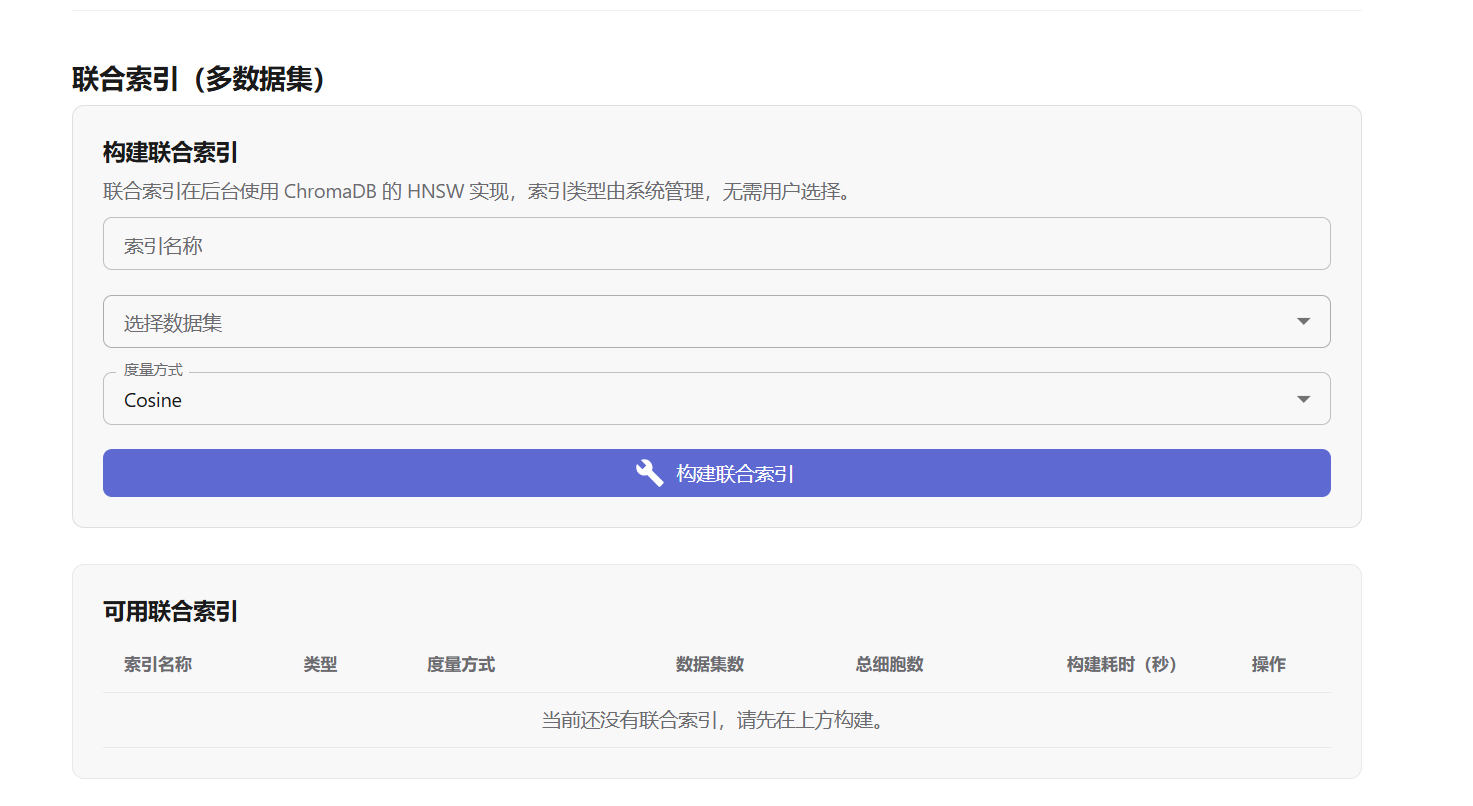
\includegraphics[width=\textwidth,keepaspectratio]{image/联合索引管理界面.png}
      \caption{联合索引管理界面}
    \end{figure}
  \end{column}
\end{columns}

\end{frame}

% ================================================================
% 课程要求 4/6：相似细胞检索
% ================================================================
\begin{frame}{相似细胞检索}

\begin{columns}[T]
  \begin{column}{0.42\textwidth}
    \fontsize{8}{10}\selectfont
    \textbf{三种检索方式}
    \begin{itemize}
      \item \textbf{向量检索}：直接输入数值向量
      \item \textbf{按细胞 ID 检索}：以数据集中某细胞为查询
      \item \textbf{自然语言检索}：RAG 驱动的 AI 智能搜索
    \end{itemize}

    \vspace{0.5em}
    \textbf{检索参数}
    \begin{itemize}
      \item 选择已构建的 ANN 索引
      \item 设置 Top-K（1--1000）
      \item 可选元数据过滤条件\\（cell\_type、disease、AgeGroup、donor\_id）
    \end{itemize}

    \begin{alertblock}{$\checkmark$ 课程要求 4/6}
      相似细胞检索
    \end{alertblock}
  \end{column}

  \begin{column}{0.55\textwidth}
    \begin{figure}
      \centering
      % ================================================================
      % 【截图8】搜索面板
      % ================================================================
      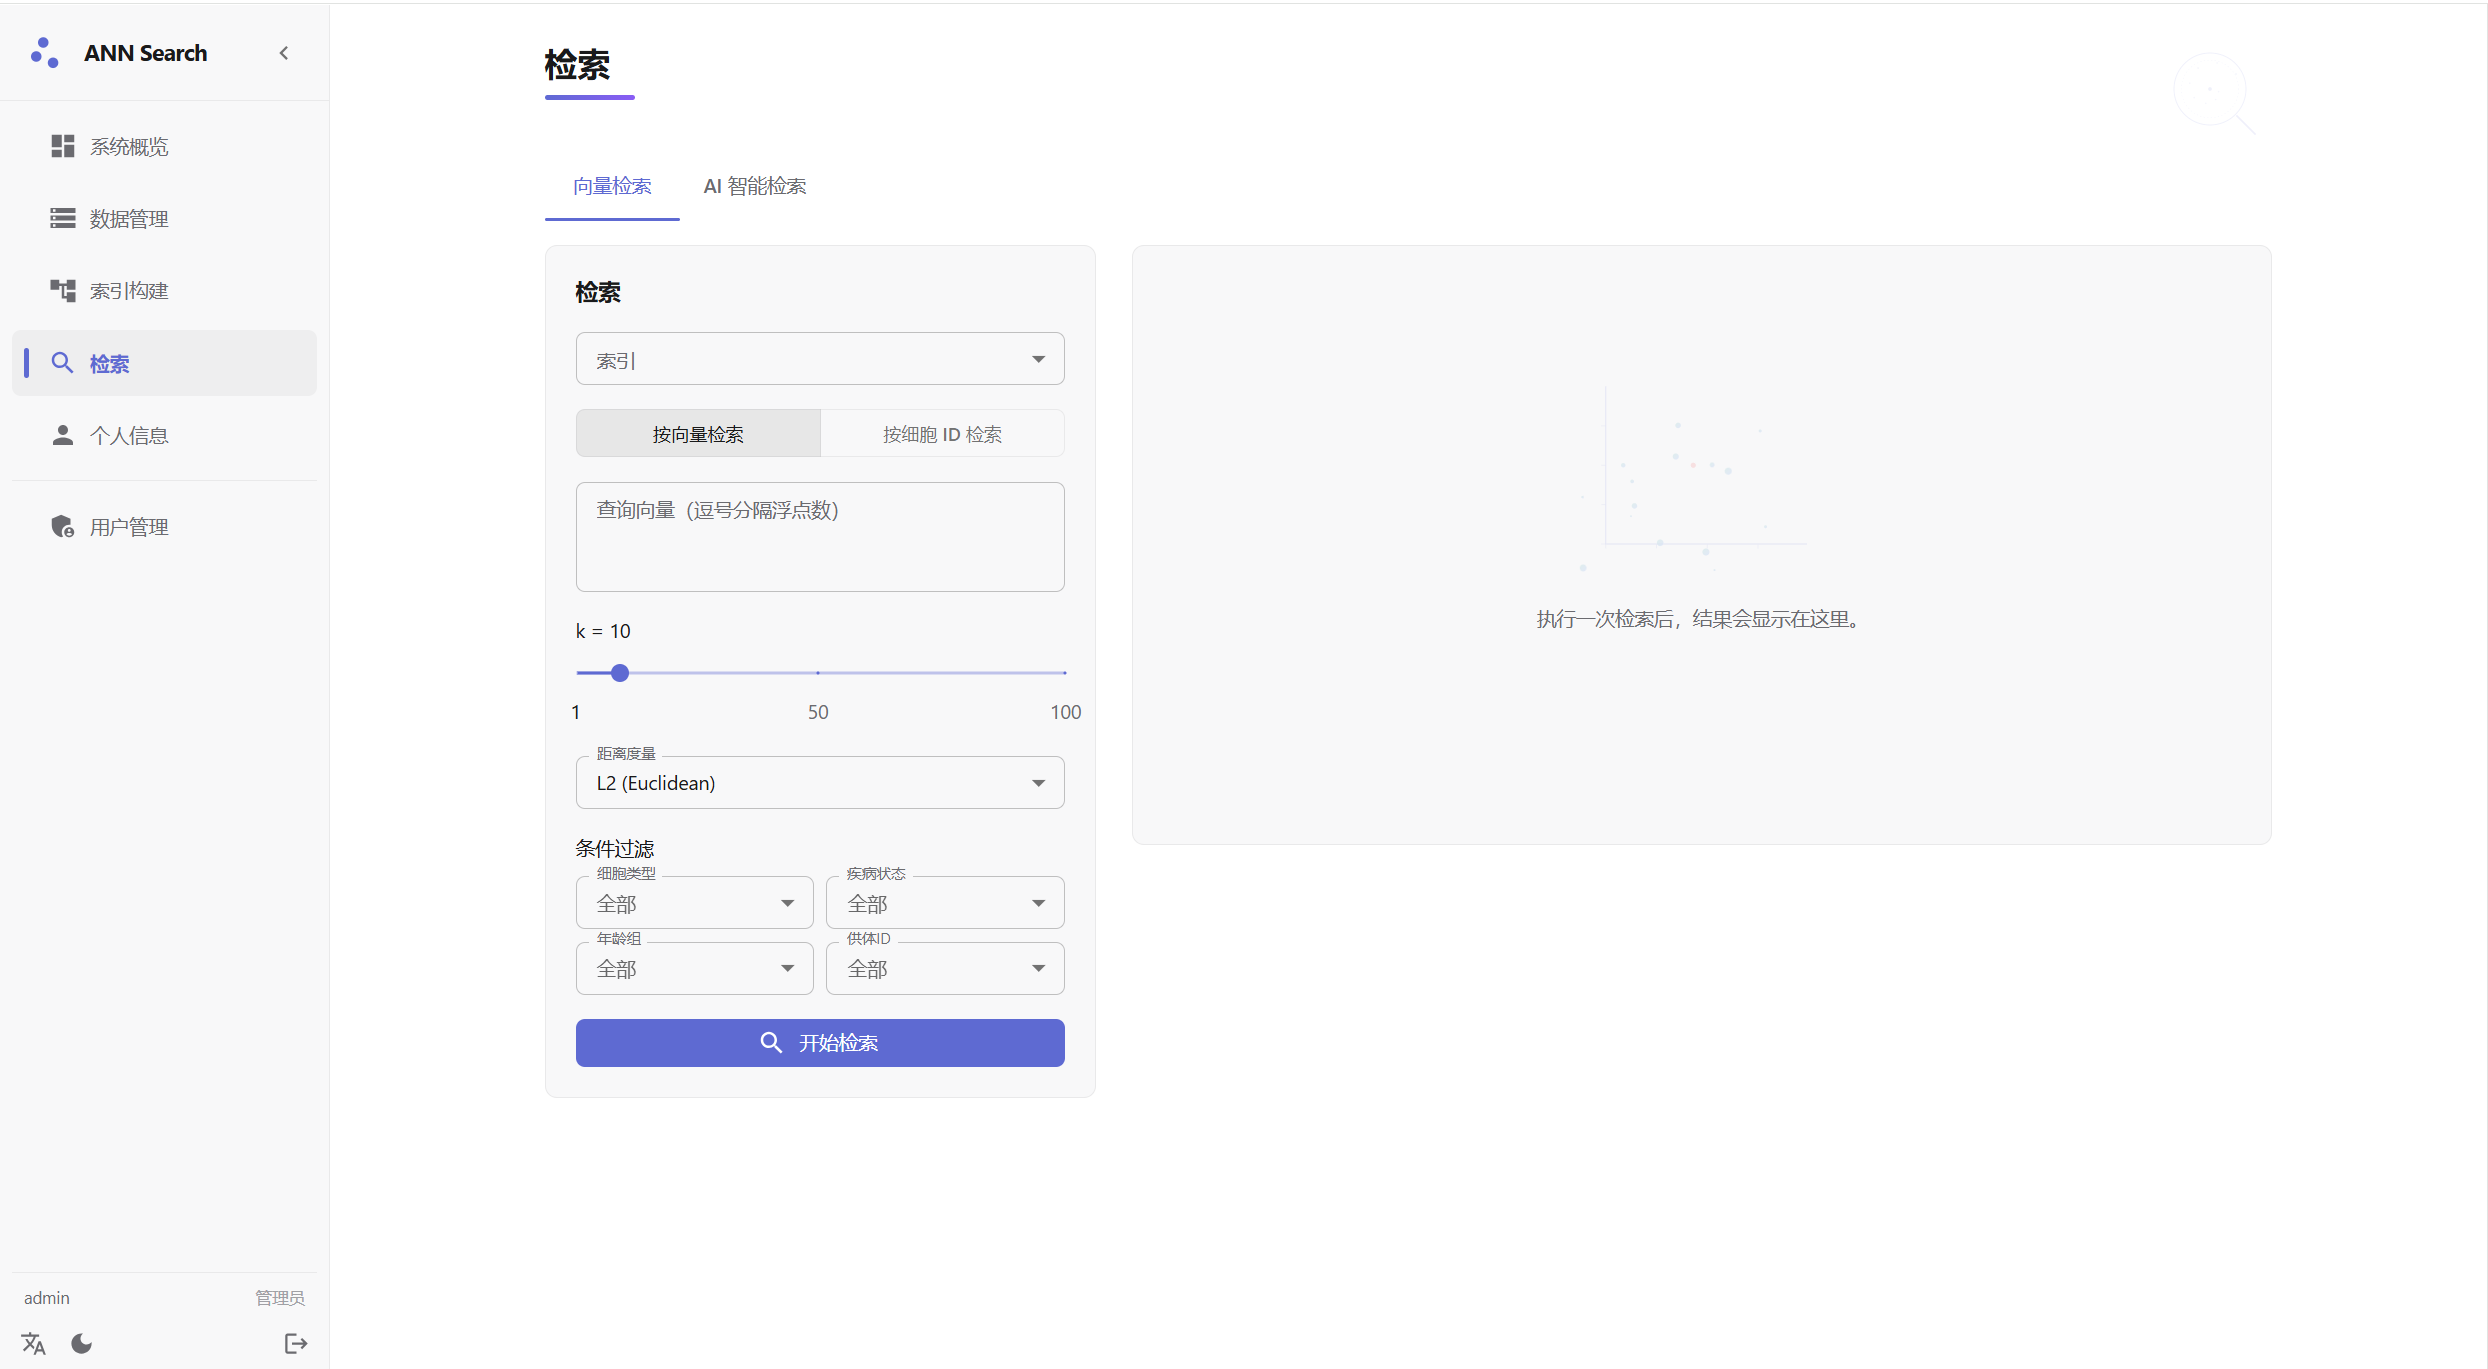
\includegraphics[width=\textwidth,keepaspectratio]{image/搜索面板.png}
      \caption{搜索面板}
    \end{figure}
  \end{column}
\end{columns}

\end{frame}

% ================================================================
% 课程要求 5/6：至少实现一种 ANN 算法或检索库
% ================================================================
\begin{frame}{实现的 ANN 算法与检索库}
\fontsize{8}{10}\selectfont

\vspace{0.3em}
\textbf{系统实现了 3 种 ANN 索引类型 + 1 种联合索引引擎，覆盖主流方案：}

\vspace{0.3em}
\begin{columns}[T]
  \begin{column}{0.48\textwidth}
    \textbf{FAISS Flat（Facebook AI Similarity Search）}
    \begin{itemize}
      \item 暴力搜索，遍历全部向量，返回\textbf{精确 Top-K}
      \item 适合小规模数据集（<10 万细胞），100\% 召回率
      \item 底层 C++ 实现，单机 CPU 即可运行
    \end{itemize}

    \vspace{0.3em}
    \textbf{ChromaDB HNSW（联合索引引擎）}
    \begin{itemize}
      \item 分层可导航小世界图（HNSW），搜索复杂度 $O(\log N)$
      \item 多数据集合并为一个 Collection，支持跨数据集检索
      \item 配合 RAG 模块实现自然语言语义搜索
    \end{itemize}
  \end{column}

  \begin{column}{0.48\textwidth}
    \textbf{Annoy（Approximate Nearest Neighbors Oh Yeah）}
    \begin{itemize}
      \item 基于随机投影树，递归划分向量空间
      \item n\_trees 控制索引精度（树越多越精确，构建越慢）
      \item 内存映射加载，无需全部读入内存
    \end{itemize}

    \vspace{0.3em}
    \textbf{FAISS IVF（Inverted File Index）}
    \begin{itemize}
      \item 倒排索引：先用 KMeans 聚类划分空间，搜索时仅扫描邻近聚类
      \item nlist 参数自动计算（$\sqrt{N}$），平衡速度与精度
      \item 适合中等至大规模数据集
    \end{itemize}
  \end{column}
\end{columns}

\vspace{0.3em}
\begin{alertblock}{$\checkmark$ 课程要求 5/6}
  至少实现一种 ANN 算法或检索库 —— 已实现 3 种 ANN 索引 + ChromaDB HNSW 联合索引
\end{alertblock}

\end{frame}

% ================================================================
% 课程要求 6/6：Top-K 相似细胞搜索，返回对应细胞信息
% ================================================================
\begin{frame}{Top-K 相似细胞搜索}

\begin{columns}[T]
  \begin{column}{0.42\textwidth}
    \fontsize{8}{10}\selectfont
    \vspace{0.5em}

    \textbf{Top-K 检索}
    \begin{itemize}
      \item 返回 \textbf{Top-K} 个最相似细胞（K 值 1--1000 可调）
      \item 每条结果包含：\textbf{排序序号、细胞名称、距离值、全部元数据}
      \item 显示\textbf{查询耗时}（ms），直观反映索引性能
      \item 支持 \textbf{CSV 一键导出}检索结果
    \end{itemize}

    \vspace{0.5em}
    \textbf{结果可视化}
    \begin{itemize}
      \item Recharts \textbf{距离分布柱状图}：直观对比各候选细胞距离
      \item 当前活跃的\textbf{过滤条件标签}：实时显示 cell\_type、disease 等筛选条件
    \end{itemize}
  \end{column}

  \begin{column}{0.55\textwidth}
    \begin{figure}
      \centering
      % ================================================================
      % 【截图9】搜索结果 + 距离分布图
      % ================================================================
      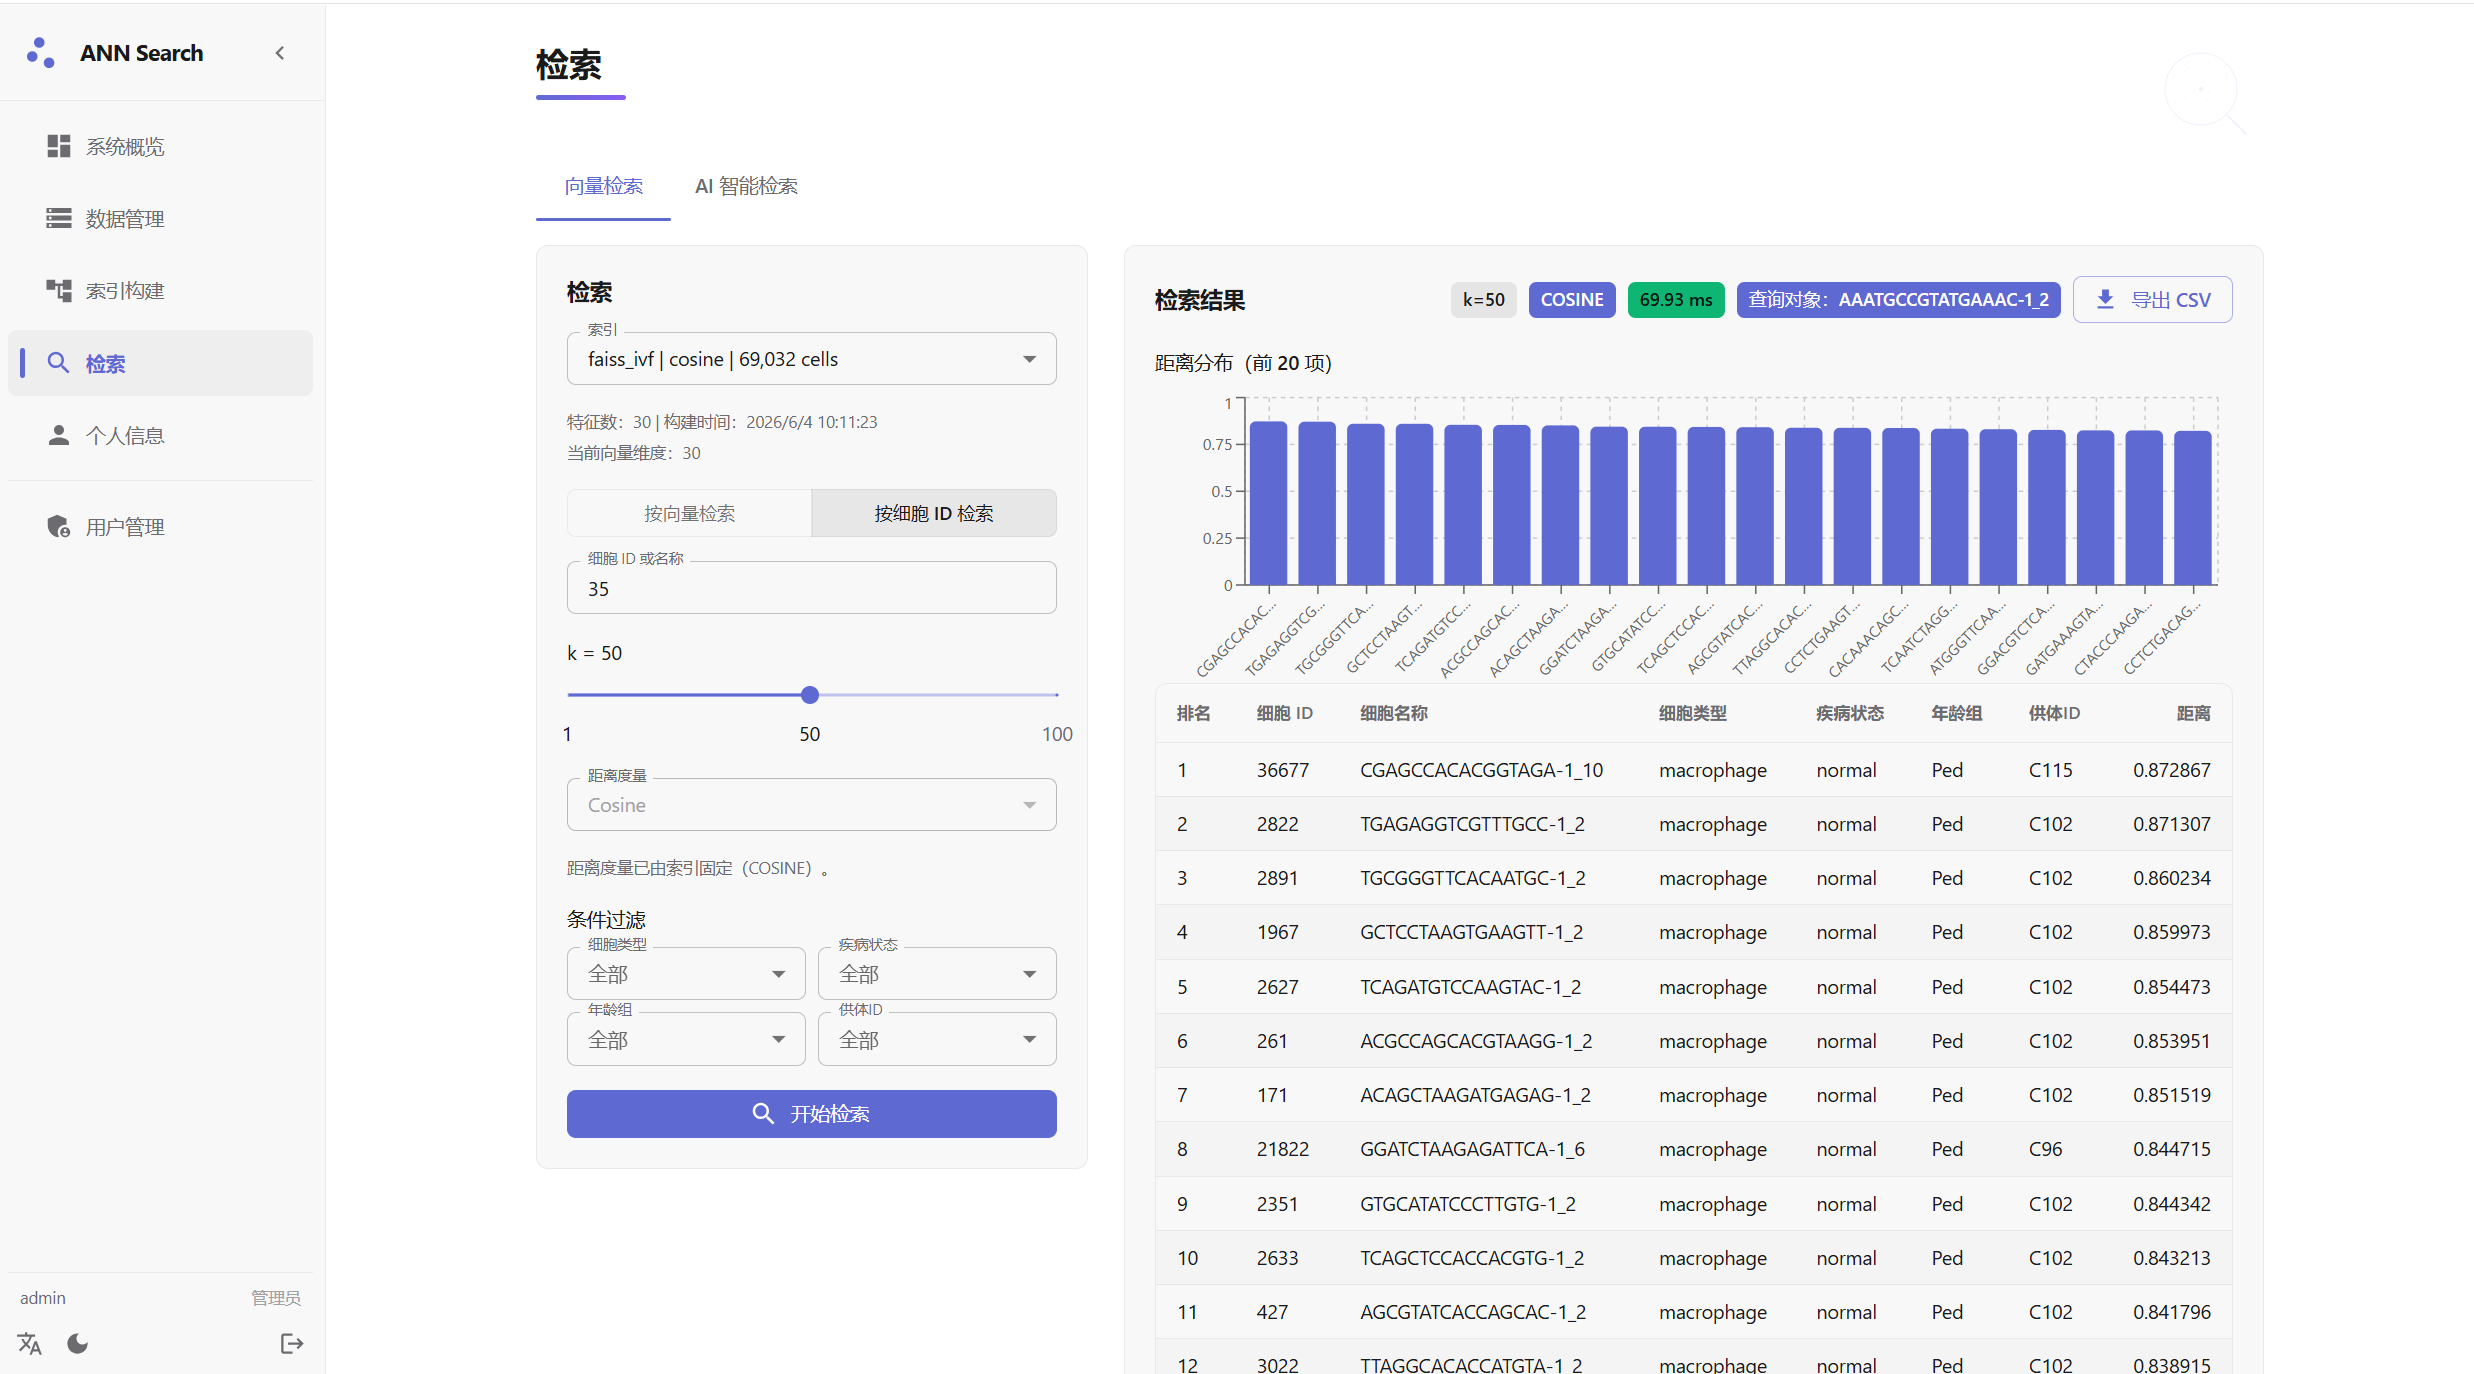
\includegraphics[width=\textwidth,keepaspectratio]{image/检索结果展示.png}
      \caption{检索结果展示}
    \end{figure}
  \end{column}
\end{columns}

\end{frame}

% ================================================================
% 搜索历史与数据导出
% ================================================================
\begin{frame}{搜索历史与数据导出}

\begin{columns}[T]
  \begin{column}{0.48\textwidth}
    \fontsize{8}{10}\selectfont
    \vspace{0.5em}

    \textbf{搜索历史管理}
    \begin{itemize}
      \item 自动保存最近 \textbf{10 条}搜索记录
      \item 记录类型：向量检索、按细胞 ID 检索、RAG 检索
      \item 支持\textbf{单条删除}、\textbf{批量删除}、\textbf{一键清空}
      \item 清空需要输入确认原因，防止误操作
    \end{itemize}

    \vspace{0.5em}
    \textbf{CSV 数据导出}
    \begin{itemize}
      \item 检索结果一键导出为 CSV 文件
      \item 包含排名、细胞 ID、细胞名称、距离值等全部字段
      \item 支持中英文列名（根据界面语言自动切换）
    \end{itemize}
  \end{column}

  \begin{column}{0.48\textwidth}
    \centering
    \begin{alertblock}{$\checkmark$ 课程要求 6/6}
      支持 Top-K 相似细胞搜索，并返回对应细胞信息
    \end{alertblock}

    \vspace{1em}
    \textbf{完整检索链路}
    \begin{center}
      \footnotesize
      选择索引 $\to$ 输入向量/细胞ID $\to$ 设置K值/过滤条件 $\to$ 发起检索 $\to$\\
      返回Top-K结果 $\to$ 图表可视化 $\to$ CSV导出 $\to$ 记录历史
    \end{center}
  \end{column}
\end{columns}

\end{frame}

% ================================================================
% 三种距离度量方式
% ================================================================
\begin{frame}{三种距离度量方式}
\small

\vspace{0.3em}
\begin{center}
（系统支持三种距离度量，构建索引时选定，搜索时锁定）
\end{center}

\vspace{0.3em}
\hspace{-1cm}
\ThreeLineTable{%
  \begin{tabular}{p{2.5cm} p{4cm} p{4cm} p{3cm}}
    \toprule
    \textbf{度量方式} & \textbf{数学含义} & \textbf{实现细节} & \textbf{选用建议} \\
    \midrule
    L2 (Euclidean)
    & $\sqrt{\sum_i(A_i-B_i)^2}$，空间直线距离
    & FAISS IndexFlatL2，Annoy euclidean
    & 数值归一化后 \\
    \hline
    Cosine
    & $\frac{A\cdot B}{|A||B|}$，方向夹角
    & L2归一化 + FAISS IndexFlatIP，Annoy angular
    & $\checkmark$ \textbf{推荐}：不受表达量影响 \\
    \hline
    Inner Product
    & $\sum_i A_i B_i$，点积大小
    & FAISS IndexFlatIP / METRIC\_INNER\_PRODUCT，Annoy dot
    & 有语义的内积场景 \\
    \bottomrule
  \end{tabular}
}

\vspace{0.5em}
\begin{block}{为什么 Cosine 是单细胞分析的默认选择？}
  基因表达量受测序深度影响大，余弦相似度关心\textbf{基因相对表达模式的方向相似性}，不受总量影响。
  L2 归一化后 Cosine $\equiv$ Inner Product，因此在 FAISS 中实际用内积索引实现余弦检索。
\end{block}

\vspace{0.3em}
\begin{itemize}
  \item 三种度量均覆盖 FAISS Flat、FAISS IVF、Annoy 三种索引类型
  \item 联合索引（ChromaDB HNSW）额外支持 cosine / l2 / ip 三种 space
\end{itemize}

\end{frame}

% ================================================================
% 项目统计
% ================================================================
\begin{frame}{项目规模统计}

\begin{columns}[T]
  \begin{column}{0.48\textwidth}
    \centering
    \textbf{\large 后端规模}

    \vspace{0.3em}
    \fontsize{8}{10}\selectfont
    \ThreeLineTable{%
      \begin{tabular}{lr}
        \toprule
        \textbf{模块} & \textbf{数量} \\
        \midrule
        API 端点 & 25+ \\
        路由蓝图 & 8 个 \\
        ANN 索引类型 & 3 种 \\
        距离度量 & 3 种 \\
        数据格式支持 & 4 种 \\
        \bottomrule
      \end{tabular}
    }

    \vspace{0.5em}
    \textbf{ANN 算法/检索库}
    \begin{itemize}
      \item FAISS Flat、FAISS IVF、Annoy
      \item ChromaDB HNSW（联合索引）
      \item 三种度量 × 三种索引 = 9 种组合
    \end{itemize}
  \end{column}

  \begin{column}{0.48\textwidth}
    \centering
    \textbf{\large 前端规模}

    \vspace{0.3em}
    \fontsize{8}{10}\selectfont
    \ThreeLineTable{%
      \begin{tabular}{lr}
        \toprule
        \textbf{模块} & \textbf{数量} \\
        \midrule
        页面 & 7 个 \\
        组件 & 13 个 \\
        i18n 语言 & 中/英 \\
        图表库 & Recharts \\
        UI 框架 & Material UI 5 \\
        \bottomrule
      \end{tabular}
    }

    \vspace{0.5em}
    \textbf{关键功能覆盖}
    \begin{itemize}
      \item 6 项课程要求全部完成
      \item RAG 检索 + 联合索引
      \item JWT 认证 + 管理员系统
      \item 中英文切换 + 深色/浅色主题
    \end{itemize}
  \end{column}
\end{columns}

\end{frame}

%%%%%%%%%%%%%%%%%%%%%%%%%%%%%%%%%%%%%%%%%%%%%%%%%%%%%%%%%%
% 过渡页：RAG 检索与用户权限管理
%%%%%%%%%%%%%%%%%%%%%%%%%%%%%%%%%%%%%%%%%%%%%%%%%%%%%%%%%%
\DrawTOC[3]{
  项目背景与系统架构,
  核心功能实现,
  RAG 检索与用户权限管理,
  总结与后续计划
}

%%%%%%%%%%%%%%%%%%%%%%%%%%%%%%%%%%%%%%%%%%%%%%%%%%%%%%%%%%
% AI 智能检索（RAG）
%%%%%%%%%%%%%%%%%%%%%%%%%%%%%%%%%%%%%%%%%%%%%%%%%%%%%%%%%%
\begin{frame}{AI 智能检索}

\begin{columns}[T]
  \begin{column}{0.45\textwidth}
    \fontsize{8}{10}\selectfont
    \textbf{RAG 自然语言检索流程}
    \begin{enumerate}
      \item 用户输入自然语言\\（如"找与肝癌细胞相似的 T 细胞"）
      \item Sentence-Transformers 编码语义
      \item 自动提取元数据过滤条件
      \item ChromaDB HNSW 语义搜索
      \item AI 生成结果\textbf{统计分析与自然语言解读}
    \end{enumerate}
  \end{column}

  \begin{column}{0.52\textwidth}
    \begin{figure}
      \centering
      % ================================================================
      % 【截图10】AI 搜索面板 + 分析结果
      % ================================================================
      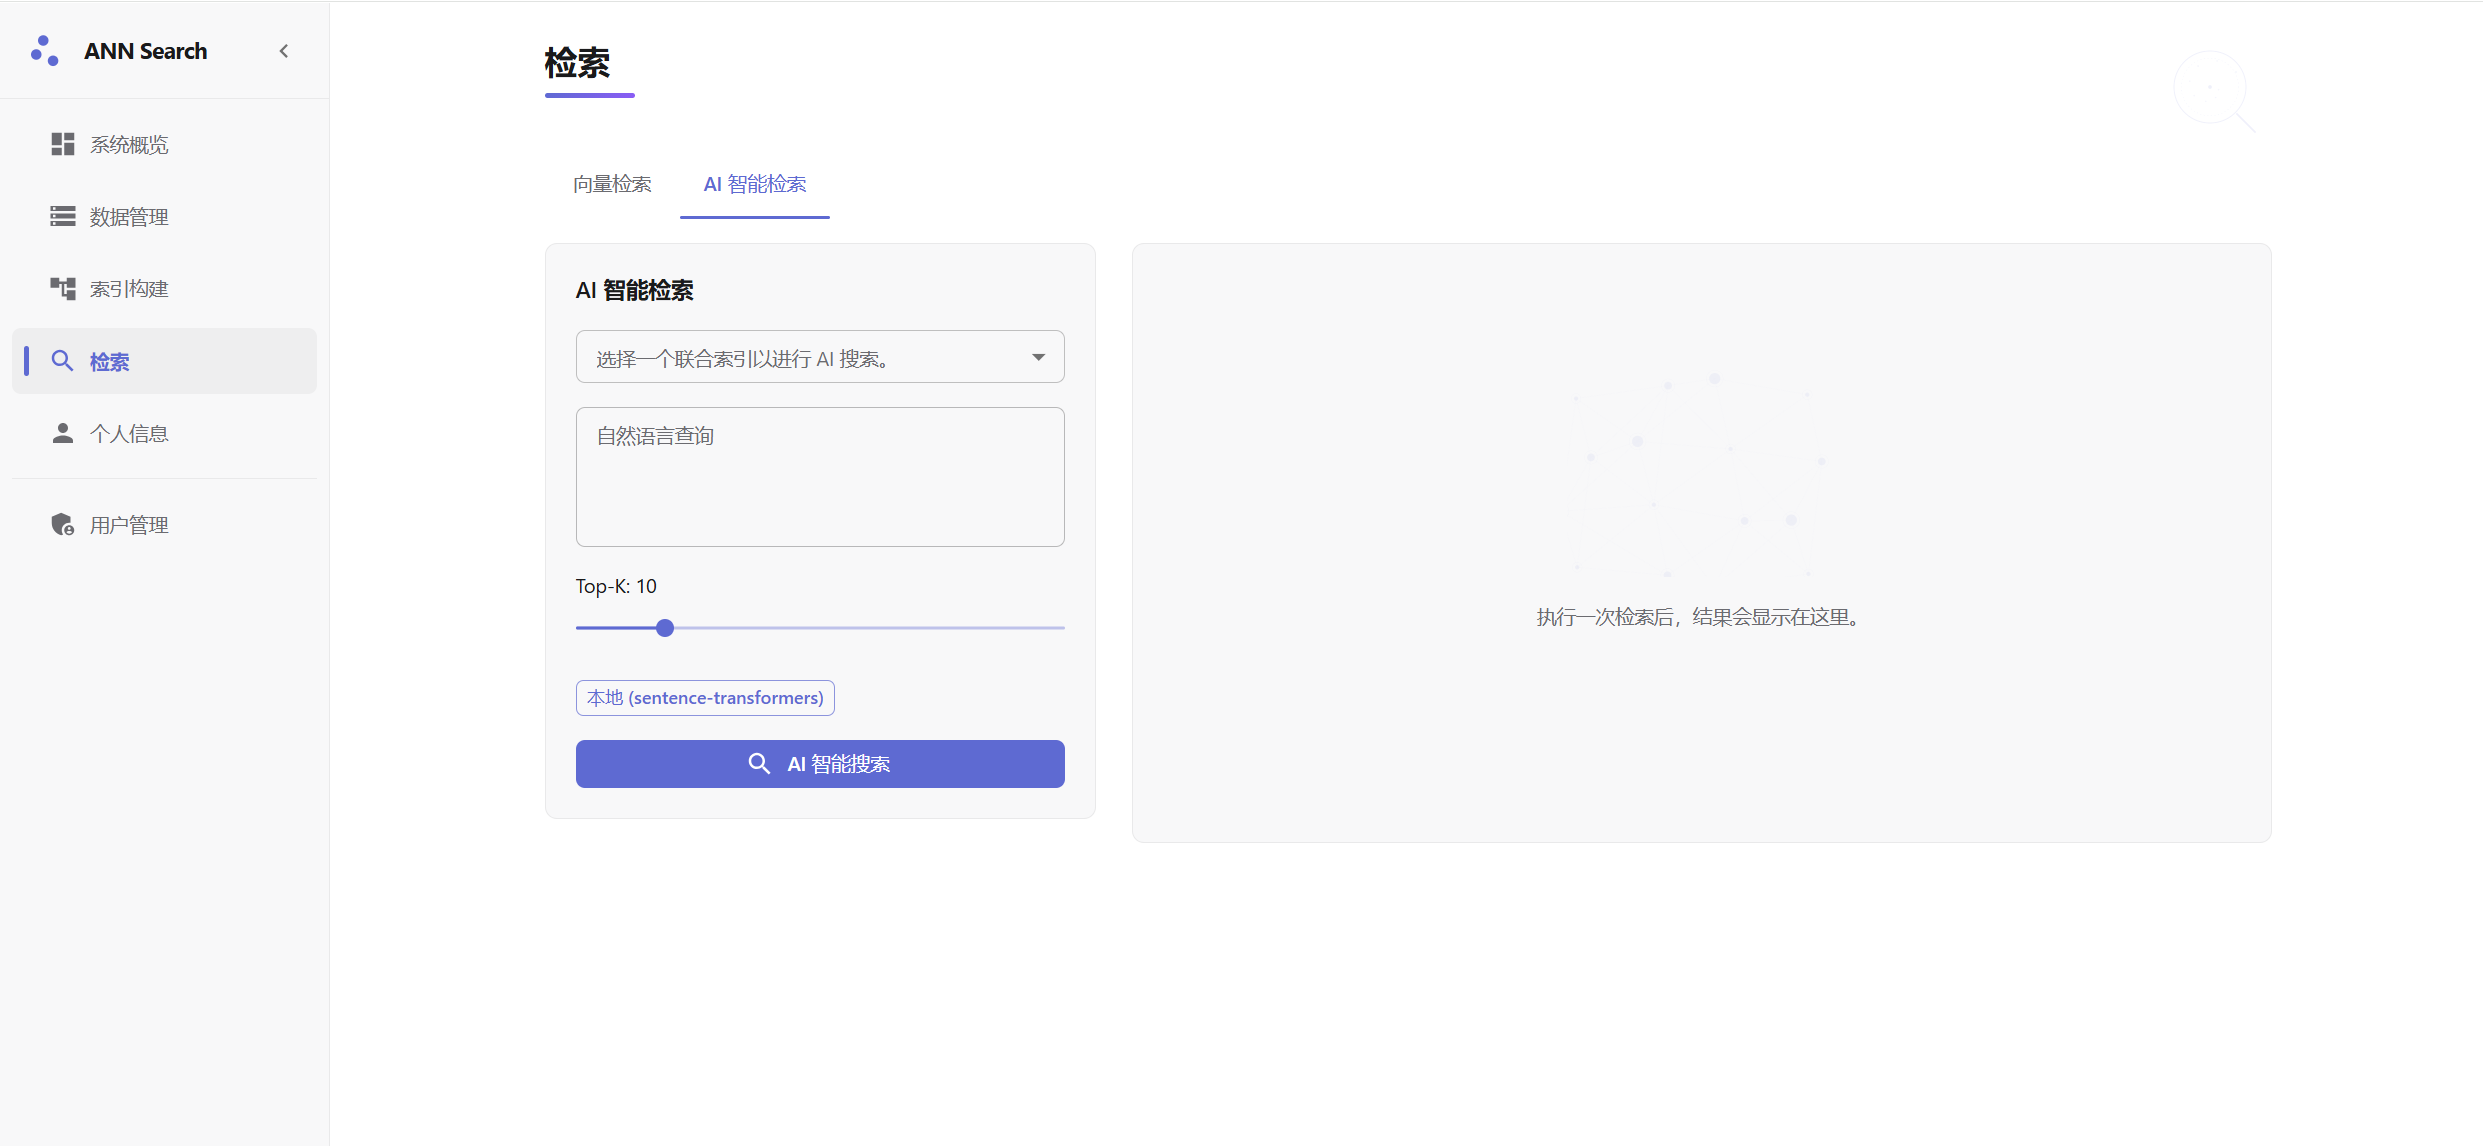
\includegraphics[width=\textwidth,keepaspectratio]{image/AI智能检索.png}
      \caption{AI 智能检索}
    \end{figure}
  \end{column}
\end{columns}

\end{frame}

%%%%%%%%%%%%%%%%%%%%%%%%%%%%%%%%%%%%%%%%%%%%%%%%%%%%%%%%%%
% 个人资料管理
%%%%%%%%%%%%%%%%%%%%%%%%%%%%%%%%%%%%%%%%%%%%%%%%%%%%%%%%%%
\begin{frame}{个人资料管理}

\begin{columns}[T]
  \begin{column}{0.45\textwidth}
    \fontsize{8}{10}\selectfont
    \textbf{Profile 页面功能}
    \begin{itemize}
      \item 查看与修改\textbf{用户名、邮箱}
      \item 修改密码（需验证旧密码）
      \item 账户信息实时更新
    \end{itemize}

    \vspace{0.5em}
    \textbf{JWT 认证机制}
    \begin{itemize}
      \item 注册：用户名 + 邮箱 + 密码
      \item 登录：返回 JWT access token
      \item 所有 API 受 \texttt{@jwt\_required()} 保护
    \end{itemize}
  \end{column}

  \begin{column}{0.52\textwidth}
    \begin{figure}
      \centering
      % ================================================================
      % 【截图11】个人资料管理页面
      % ================================================================
      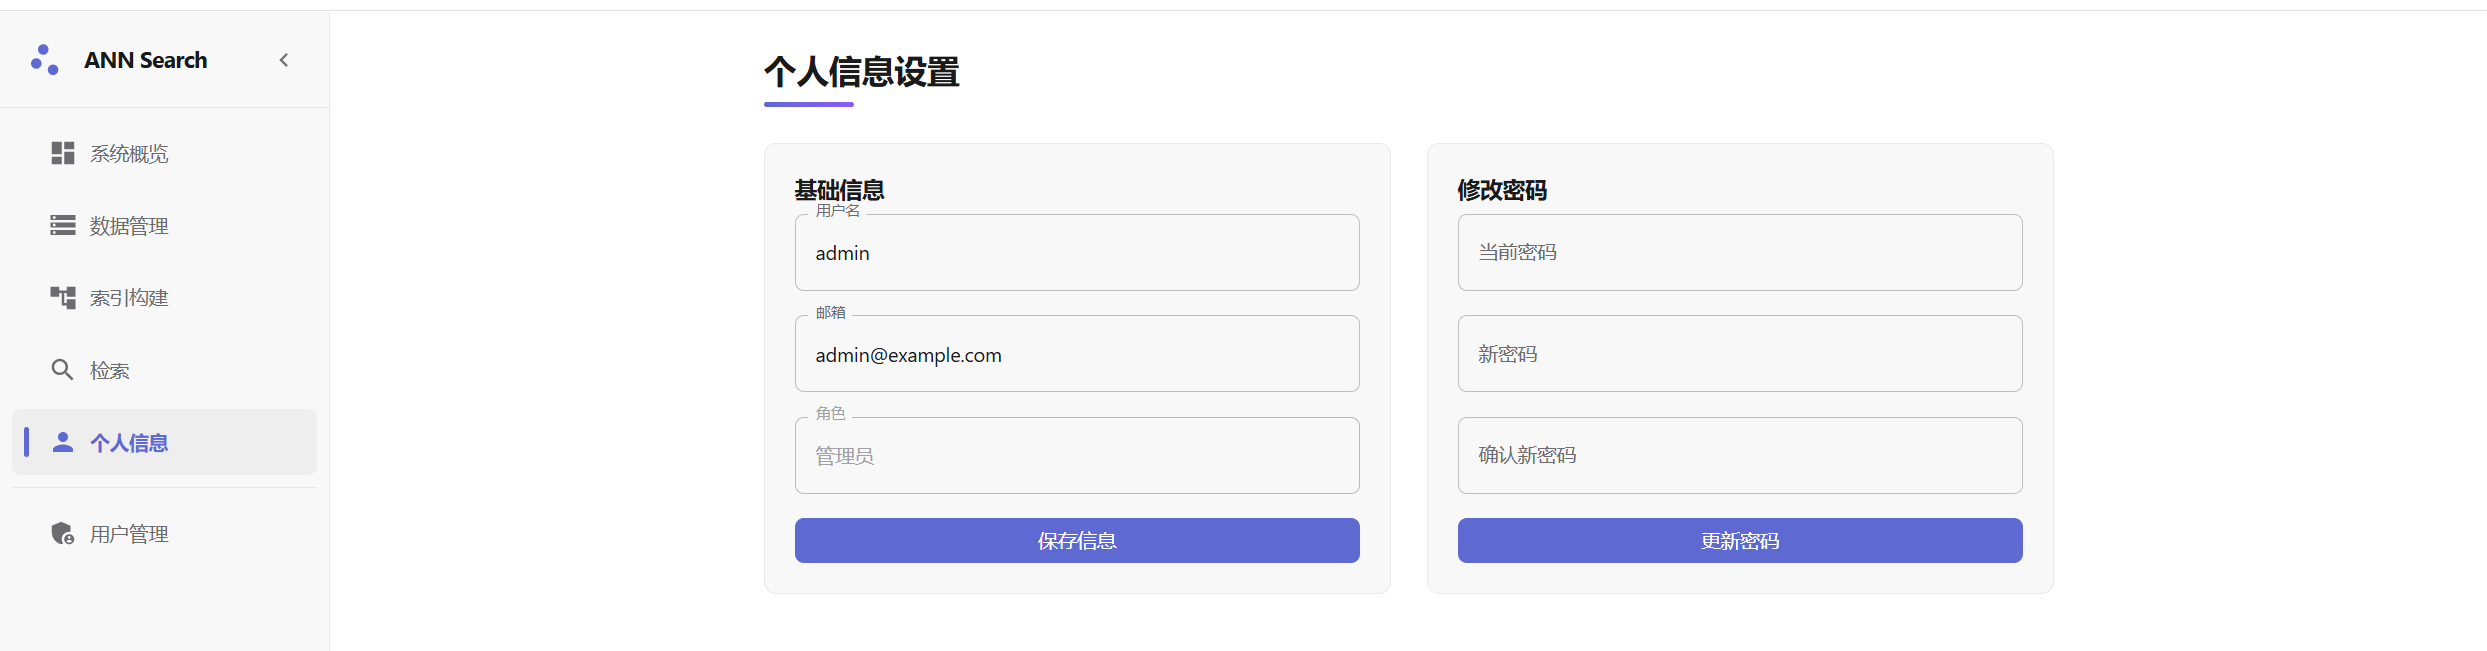
\includegraphics[width=\textwidth,keepaspectratio]{image/个人资料管理.png}
      \caption{个人资料管理}
    \end{figure}
  \end{column}
\end{columns}

\end{frame}

%%%%%%%%%%%%%%%%%%%%%%%%%%%%%%%%%%%%%%%%%%%%%%%%%%%%%%%%%%
% 用户认证与管理员功能
%%%%%%%%%%%%%%%%%%%%%%%%%%%%%%%%%%%%%%%%%%%%%%%%%%%%%%%%%%
\begin{frame}{用户认证与权限管理}

\begin{columns}[T]
  \begin{column}{0.45\textwidth}
    \fontsize{8}{10}\selectfont
    \vspace{1.5em}

    \textbf{管理员功能（Admin）}
    \begin{itemize}
      \item 查看所有普通用户列表
      \item 创建新用户、编辑用户信息
      \item 重置用户密码、删除用户
      \item 管理员账户通过 \texttt{.env} 自动初始化
    \end{itemize}

    \vspace{0.5em}
    \textbf{中英文界面切换}
    \begin{itemize}
      \item 完整的 i18n 翻译支持
      \item 导航栏一键切换语言
    \end{itemize}
  \end{column}

  \begin{column}{0.52\textwidth}
    \begin{figure}
      \centering
      % ================================================================
      % 【截图12】登录/注册界面
      % ================================================================
      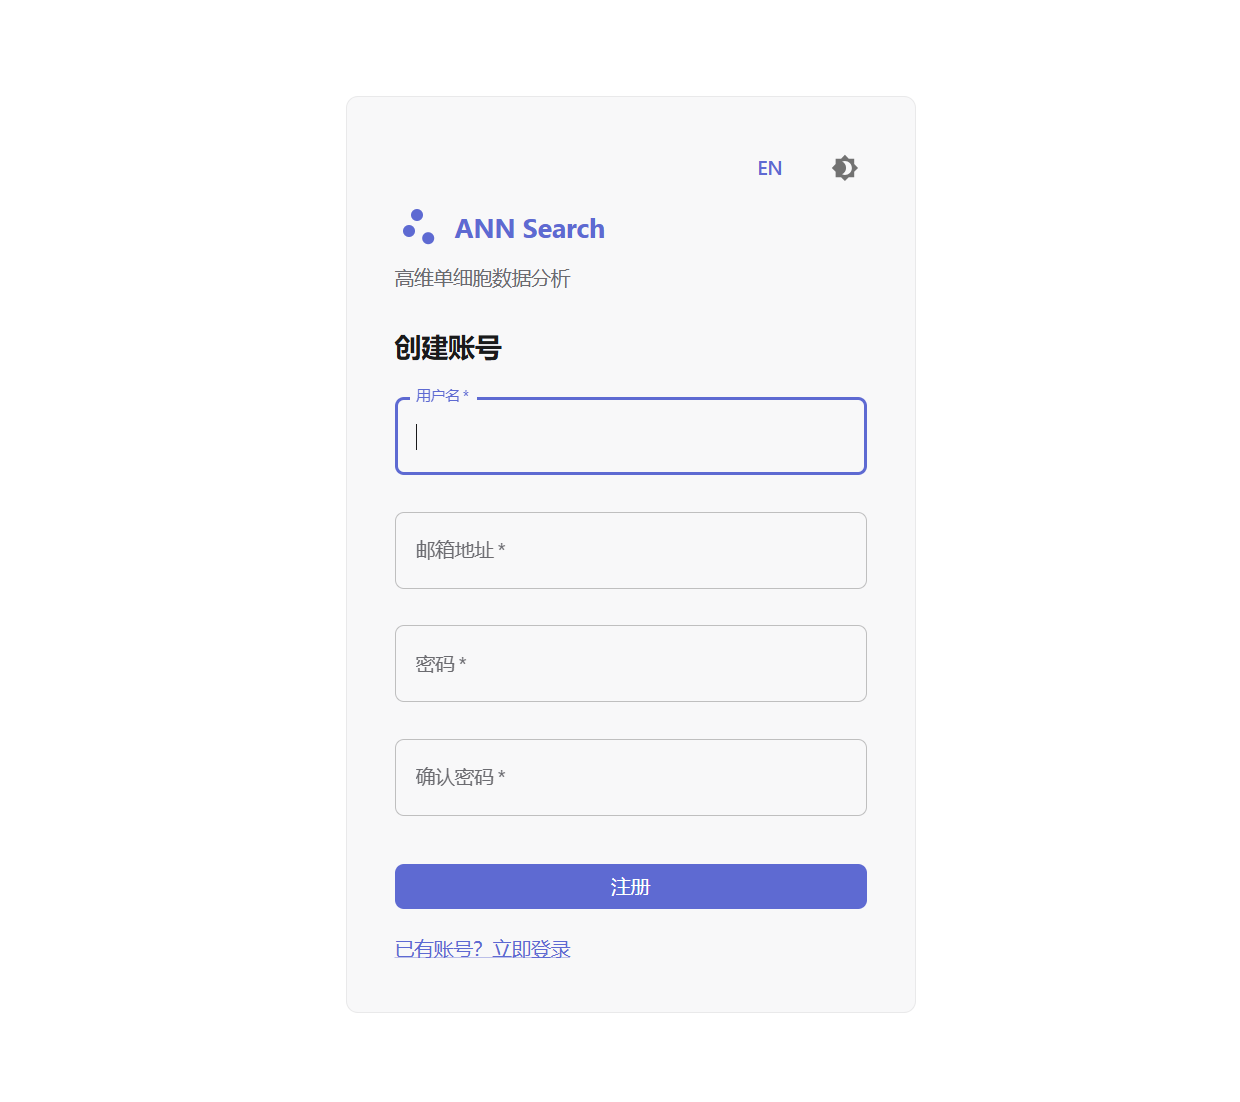
\includegraphics[width=\textwidth,keepaspectratio]{image/注册页面.png}
      \caption{登录/注册界面}

      \vspace{0.3em}
      % ================================================================
      % 【截图13】管理员用户管理页面
      % ================================================================
      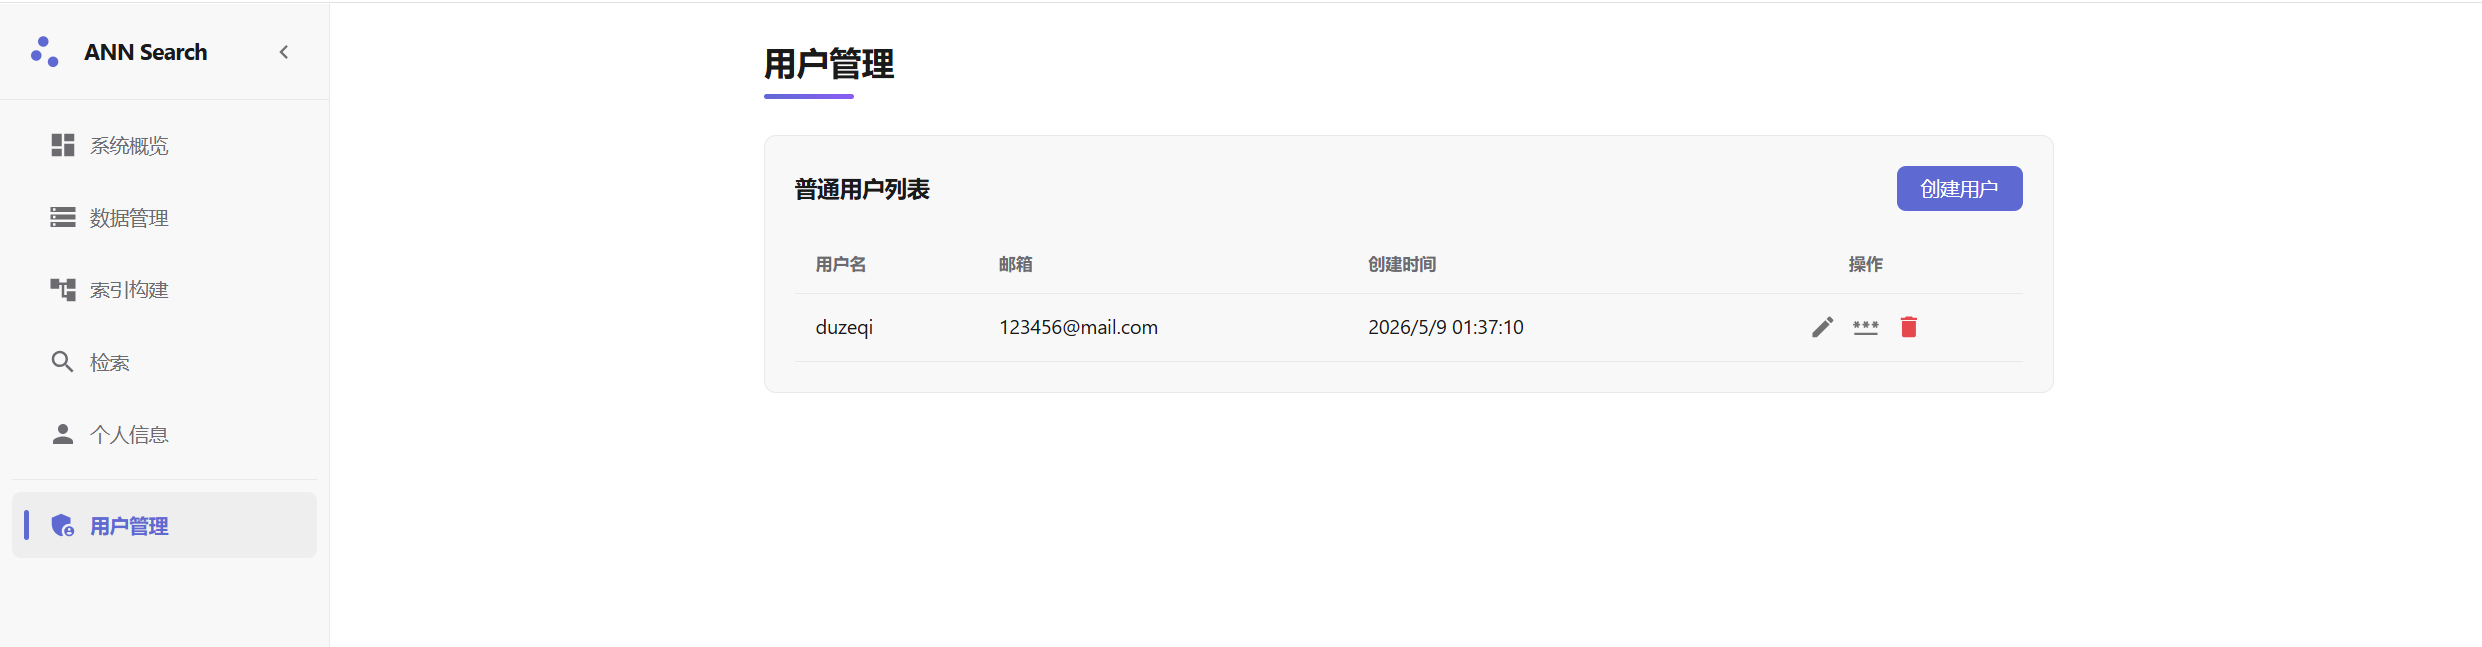
\includegraphics[width=\textwidth,keepaspectratio]{image/管理员用户管理.png}
      \caption{管理员用户管理}
    \end{figure}
  \end{column}
\end{columns}

\end{frame}

%%%%%%%%%%%%%%%%%%%%%%%%%%%%%%%%%%%%%%%%%%%%%%%%%%%%%%%%%%
% 过渡页：总结与后续计划
%%%%%%%%%%%%%%%%%%%%%%%%%%%%%%%%%%%%%%%%%%%%%%%%%%%%%%%%%%
\DrawTOC[4]{
  项目背景与系统架构,
  核心功能实现,
  RAG 检索与用户权限管理,
  总结与后续计划
}

%%%%%%%%%%%%%%%%%%%%%%%%%%%%%%%%%%%%%%%%%%%%%%%%%%%%%%%%%%
% 总结与后续计划
%%%%%%%%%%%%%%%%%%%%%%%%%%%%%%%%%%%%%%%%%%%%%%%%%%%%%%%%%%
\begin{frame}{总结与后续计划}
\small

\begin{block}{中期已完成——六项课程要求全覆盖}
  \begin{itemize}
    \item \textbf{单细胞数据读取}：支持 CSV/TSV/HDF5/H5AD，含课程 liver 数据适配
    \item \textbf{数据向量化表示}：PCA 嵌入 + L2 归一化 + z-score 标准化
    \item \textbf{ANN 索引构建}：FAISS Flat、FAISS IVF、Annoy（3 种）+ ChromaDB 联合索引
    \item \textbf{相似细胞检索}：向量检索 / 按细胞 ID 检索 / RAG 自然语言检索
    \item \textbf{至少一种 ANN 算法}：实现 3 种 ANN 索引 + ChromaDB 联合索引，远超最低要求
    \item \textbf{Top-K + 返回细胞信息}：Top-K 可调，返回排序序号、细胞名称、距离值、全部元数据、查询耗时
  \end{itemize}
\end{block}

\vspace{0.2em}
\begin{exampleblock}{附加功能}
  RAG AI 智能检索 · 多数据集联合索引 · JWT 用户认证 · 管理员系统 · 距离分布可视化 · CSV 导出 · 搜索历史管理 · 中英文切换
\end{exampleblock}

\vspace{0.2em}
\begin{exampleblock}{后续计划}
  性能评测（Recall@K）· 大规模 liver 数据测试 · 文档完善 · 结项报告与演示视频
\end{exampleblock}

\end{frame}

%%%%%%%%%%%%%%%%%%%%%%%%%%%%%%%%%%%%%%%%%%%%%%%%%%%%%%%%%%
% Q&A 页
%%%%%%%%%%%%%%%%%%%%%%%%%%%%%%%%%%%%%%%%%%%%%%%%%%%%%%%%%%
\begin{frame}{提问与解答}
  \centering
  \vspace{0.8cm}
  {\Huge {\bfseries Q\&A} \\
  \vspace{0.25em} \Large 感谢聆听，欢迎提问}

  \vspace{1.5cm}
  \normalsize 软件工程 第13组
\end{frame}

%%%%%%%%%%%%%%%%%%%%%%%%%%%%%%%%%%%%%%%%%%%%%%%%%%%%%%%%%%
% 致谢页
%%%%%%%%%%%%%%%%%%%%%%%%%%%%%%%%%%%%%%%%%%%%%%%%%%%%%%%%%%
\begin{frame}[plain]
  \begin{tikzpicture}[remember picture,overlay]
    \node[fill=midpurple, opacity=1, minimum width=\paperwidth, minimum height=\paperheight] at (current page.center) {};
    \node[font=\fontsize{40}{70}\selectfont\bfseries, text=white] at (current page.center) {致谢};
  \end{tikzpicture}
\end{frame}

\end{document}
